\documentclass[12pt]{article}
\RequirePackage{amsthm,amsmath,amsbsy,amsfonts}
\usepackage{bbm}
\usepackage{bm,graphicx,psfrag,epsf}
%\usepackage{enumerate}
\usepackage{natbib}
\usepackage{url} % not crucial - just used below for the URL 
\usepackage{placeins}
\usepackage{algorithm}
\usepackage{algpseudocode}
\usepackage{subfig} %% For \subfloat command

\newtheorem{proposition}{Proposition}[section]


%\pdfminorversion=4
% NOTE: To produce blinded version, replace "0" with "1" below.
\newcommand{\blind}{0}

% DON'T change margins - should be 1 inch all around.
\addtolength{\oddsidemargin}{-.5in}%
\addtolength{\evensidemargin}{-.5in}%
\addtolength{\textwidth}{1in}%
\addtolength{\textheight}{1.3in}%
\addtolength{\topmargin}{-.8in}%

\usepackage[usenames]{color}
\usepackage{xspace}

%% For comments to each other
\definecolor{blue}{rgb}{0.2,0.5,0.7}
\definecolor{green}{rgb}{0.3,0.68,0.29}
\definecolor{purple}{rgb}{0.6,0.31,0.64}
\newcommand{\Halley}[2]{{\bf {\color{purple}@Halley from #1: #2}}\xspace}
\newcommand{\Joe}[2]{{\bf {\color{blue}@Joe from #1: #2}}\xspace}
\newcommand{\Eric}[2]{{\bf {\color{green}@Eric from #1: #2}}\xspace}

%% Turn on/off options for PDF
\usepackage{ifpdf}

%% For hyperlinks. Should always be the last package. Omit for DVI version.
\ifpdf
\usepackage[colorlinks,urlcolor=blue,citecolor=blue,linkcolor=blue]{hyperref}
\else
\newcommand{\href}[2]{{#2}}
\usepackage{url}
\fi

%% ----------------------------------------------------------------------
%% Hyper-linked References
%% ----------------------------------------------------------------------

\ifpdf
\newcommand{\Sec}[1]{\hyperref[sec:#1]{Section~\ref*{sec:#1}}} %section
\newcommand{\App}[1]{\hyperref[sec:#1]{Appendix~\ref*{sec:#1}}} %appendix
\newcommand{\Eqn}[1]{\hyperref[eq:#1]{{\rm (\ref*{eq:#1})}}} %equation
\newcommand{\Part}[1]{\hyperref[part:#1]{(\ref*{part:#1})}} %part of theorem
\newcommand{\Fig}[1]{\hyperref[fig:#1]{Figure~\ref*{fig:#1}}} %figure
\newcommand{\Tab}[1]{\hyperref[tab:#1]{Table~\ref*{tab:#1}}} %table
\newcommand{\Thm}[1]{\hyperref[thm:#1]{Theorem~\ref*{thm:#1}}} %theorem
\newcommand{\Lem}[1]{\hyperref[lem:#1]{Lemma~\ref*{lem:#1}}} %lemma
\newcommand{\Prop}[1]{\hyperref[prop:#1]{Proposition~\ref*{prop:#1}}} %proposition
\newcommand{\Cor}[1]{\hyperref[cor:#1]{Corollary~\ref*{cor:#1}}} %corollary
\newcommand{\Def}[1]{\hyperref[def:#1]{Definition~\ref*{def:#1}}} %definition
\newcommand{\Alg}[1]{\hyperref[alg:#1]{Algorithm~\ref*{alg:#1}}} %algorithm
\newcommand{\Ex}[1]{\hyperref[ex:#1]{Example~\ref*{ex:#1}}} %example
\newcommand{\As}[1]{\hyperref[as:#1]{Assumption~{\rm\ref*{as:#1}}}} %assumption
\newcommand{\Reg}[1]{\hyperref[as:#1]{Condition~\ref*{reg:#1}}} %regularity condition
\newcommand{\AlgLine}[2]{\hyperref[alg:#1]{line~\ref*{line:#2} of Algorithm~\ref*{alg:#1}}}
\newcommand{\AlgLines}[3]{\hyperref[alg:#1]{lines~\ref*{line:#2}--\ref*{line:#3} of Algorithm~\ref*{alg:#1}}}
\else
\newcommand{\Sec}[1]{{Section~\ref{sec:#1}}} %section
\newcommand{\App}[1]{{Appendix~\ref{sec:#1}}} %appendix
\newcommand{\Eqn}[1]{{(\ref{eq:#1})}} %equation
\newcommand{\Part}[1]{{(\ref{part:#1})}} %part of proof
\newcommand{\Fig}[1]{{Figure~\ref{fig:#1}}} %figure
\newcommand{\Tab}[1]{{Table~\ref{tab:#1}}} %table
\newcommand{\Thm}[1]{{Theorem~\ref{thm:#1}}} %theorem
\newcommand{\Lem}[1]{{Lemma~\ref{lem:#1}}} %lemma
\newcommand{\Prop}[1]{{Property~\ref{prop:#1}}} %property
\newcommand{\Cor}[1]{{Corollary~\ref{cor:#1}}} %corollary
\newcommand{\Def}[1]{{Definition~\ref{def:#1}}} %definition
\newcommand{\Alg}[1]{{Algorithm~\ref{alg:#1}}} %algorithm
\newcommand{\Ex}[1]{{Example~\ref{ex:#1}}} %example
\newcommand{\As}[1]{{Assumption~\ref{as:#1}}} %assumption
\newcommand{\Reg}[1]{{R~\ref{reg:#1}}} %regularity condition
\newcommand{\AlgLine}[2]{{line~\ref{line:#2} of Algorithm~\ref{alg:#1}}}
\newcommand{\AlgLines}[3]{{lines~\ref{line:#2}--\ref{line:#3} of Algorithm~\ref{alg:#1}}}
\fi

%% ----------------------------------------------------------------------
%% Definitions
%% ----------------------------------------------------------------------

%% Shorthand for Real
\newcommand{\Real}{\mathbb{R}}

%% Math notation
\newcommand{\Tra}{^{\sf T}} % Transpose
\newcommand{\Inv}{^{-1}} % Inverse
\newcommand{\tr}{\operatorname{tr}} % Trace
\newcommand{\Ker}{\operatorname{Ker}} % Kernel
\def\vec{\mathop{\rm vec}\nolimits}
\newcommand{\amp}{\mathop{\:\:\,}\nolimits}
\newcommand{\bic}{\text{BIC}}
\newcommand{\ebic}{\text{eBIC}}
\newcommand{\sic}{\text{SIC}}
\newcommand{\VI}{\text{VI}}
\newcommand{\One}{\mathbbm{1}}

%% Vectors
\newcommand{\V}[1]{{\bm{\mathbf{\MakeLowercase{#1}}}}} % vector
\newcommand{\VE}[2]{\MakeLowercase{#1}_{#2}} % vector element
\newcommand{\Vbar}[1]{{\bm{\bar \mathbf{\MakeLowercase{#1}}}}} % vector
\newcommand{\Vhat}[1]{{\bm{\hat \mathbf{\MakeLowercase{#1}}}}} % vector
\newcommand{\Vtilde}[1]{{\bm{\tilde \mathbf{\MakeLowercase{#1}}}}} % vector
\newcommand{\Vn}[2]{\V{#1}^{(#2)}} % n-th vector
\newcommand{\VnE}[3]{{#1}^{(#2)}_{#3}} % n-th vector
\newcommand{\VtildeE}[2]{\tilde{\MakeLowercase{#1}}_{#2}} % vector element


%% Matrices
\newcommand{\M}[1]{{\bm{\mathbf{\MakeUppercase{#1}}}}} % matrix
\newcommand{\ME}[2]{\MakeLowercase{#1}_{#2}} % matrix element
\newcommand{\MC}[2]{\V{#1}_{#2}}
\newcommand{\Mr}[2]{\V{#1}_{#2}} % matrix row
\newcommand{\Mhat}[1]{{\bm{\hat \mathbf{\MakeUppercase{#1}}}}} % matrix
\newcommand{\Mtilde}[1]{{\bm{\tilde \mathbf{\MakeUppercase{#1}}}}} % matrix
\newcommand{\MhatC}[2]{\Vhat{#1}_{#2}} % matrix column
\newcommand{\Mbar}[1]{{\bm{bar \mathbf{\MakeUppercase{#1}}}}} % matrix
\newcommand{\MbarC}[2]{\Vbar{#1}_{#2}} % matrix column
\newcommand{\Mn}[2]{\M{#1}^{(#2)}} % n-th matrix
\newcommand{\Mbarn}[2]{\Mbar{#1}^{(#2)}} % n-th matrix
\newcommand{\Mtilden}[2]{\Mtilde{#1}^{(#2)}} % n-th matrix
\newcommand{\MnTra}[2]{\M{#1}^{(#2){{\sf T}}}} % n-th matrix transpose
\newcommand{\MnE}[3]{\MakeLowercase{#1}^{(#2)}_{#3}} % n-th matrix element
\newcommand{\MnC}[3]{\V{#1}^{(#2)}_{#3}} % n-th matrix column
\newcommand{\MbarnC}[3]{\Vbar{#1}^{(#2)}_{#3}} % n-th matrix column
\newcommand{\MnCTra}[3]{\V{#1}^{(#2){{\sf T}}}_{#3}} % n-th matrix column transpose
\newcommand{\MCTra}[2]{\V{#1}^{{\sf T}}_{#2}} % n-th matrix column transpose



\begin{document}
	
	%\bibliographystyle{natbib}
	
	\def\spacingset#1{\renewcommand{\baselinestretch}%
		{#1}\small\normalsize} \spacingset{1}
	
	
	%%%%%%%%%%%%%%%%%%%%%%%%%%%%%%%%%%%%%%%%%%%%%%%%%%%%%%%%%%%%%%%%%%%%%%%%%%%%%%
	
	\if0\blind
	{
		\title{\bf Baseline Drift Estimation for Time Series Data Using Quantile Trend Filtering}
		\author{Halley Brantley\thanks{
				Department of Statistics, North Carolina State University, Raleigh, NC 27695 (E-mail: hlbrantl@ncsu.edu)} \,
			Joseph Guinness\thanks{
				Department of Statistics and Data Science, Cornell University, Ithaca, NY 14853 (E-mail: guinness@cornell.edu )} \,
			and
			%    and
			Eric C. Chi\thanks{Department of Statistics, North Carolina State University, Raleigh, NC 27695 (E-mail: eric$\_$chi@ncsu.edu).}    \\}
		\date{}
		\maketitle
	} \fi
		
	\if1\blind
	{
		\bigskip
		\bigskip
		\bigskip
		\begin{center}
			{\LARGE\bf Title}
		\end{center}
		\medskip
	} \fi
	
	\bigskip
	\begin{abstract}
		We address the problem of estimating smoothly varying baseline trends in time series data using quantile trend filtering. We first extend the basic framework to ensure non-crossing while estimating multiple quantile trends simultaneously. We also implement a parallelizable alternating direction method of moments (ADMM) algorithm for estimating trends in longer series. The ADMM algorthim enables the estimation of trends in a piecewise manner, both reducing the computation time and extending the limits of the method to larger data sizes. We also address smoothing parameter selection and propose a modified criterion based on the extended Bayesian Information Criterion. Through simulation studies and an application to low cost air quality sensor data, we demonstrate that our model provides better quantile trend estimates than existing methods and improves signal classification of low-cost air quality sensor output. 
	\end{abstract}
	
	\noindent%
	{\it Keywords:} quantile regression, non-parametric regression, trend estimation, smoothing splines
	\vfill
	
	\newpage
	\spacingset{1.5} % DON'T change the spacing!
	
%% ----------------------------------------------------------------------
%% Introduction
%% ----------------------------------------------------------------------	
\section{Introduction}
\label{sec:intro}
	
In a wide range of applications that spans chemistry \citep{Ning2014}, macroeconomics \citep{yamada2017estimating}, environmental science \citep{brantley2014mobile}, and medical sciences \citep{pettersson2013algorithm, marandi2015qualitative}, scalar functions of time $y(t)$ are observed and assumed to be a superposition of an underlying slowly varying baseline trend $\theta(t)$, other more rapidly varying components $s(t)$, and noise. In practice, $y(t)$ is observed at discrete time points $t_1, \ldots, t_n$, and we model the vector of signal samples $\VE{y}{i} = y(t_i)$ as	
\begin{eqnarray*}
\V{y} & = & \V{\theta} + \V{s} + \V{\varepsilon},
\end{eqnarray*}
where $\VE{\theta}{i} = \theta(t_i)$, $\VE{s}{i} = s(t_i)$, and $\V{\varepsilon} \in \Real^n$ is a vector of uncorrelated noise. For notational simplicity, for the rest of the paper, we assume that the time points take on the values $t_i = i$, but it is straightforward to generalize to an arbitrary grid of time points.

In some applications, the slowly varying component $\V{\theta}$ is the signal of interest and the transient component $\V{s}$ is a vector of nuisance parameters. In other applications, the roles of $\V{\theta}$ and $\V{s}$ are reversed. The latter applies in the air quality applications motivating this work, as $\V{s}$ represents the signal of interest and $\V{\theta}$ represents a baseline drift that obscures the identification of the important transient events encoded in $\V{s}$. We describe this motivating problem further to illustrate the critical importance of being able to separate $\V{s}$ from $\V{\theta}$.

%	This work was motivated by the analysis of signals measured by low cost and portable air quality sensors, whose use has increased dramatically in the last decade. 
In the last decade, low cost and portable air quality sensors have enjoyed dramatically increased usage. These sensors can provide an un-calibrated measure of a variety of pollutants in near real time, but deriving meaningful information from sensor data remains a challenge \citep{snyder2013changing}. The ``SPod" is a low-cost sensor currently being investigated by researchers at the U.S. Environmental Protection Agency to detect volatile organic compound (VOC) emissions from industrial facilities \citep{thoma2016south}. To reduce cost and power consumption of the SPod, the temperature and relative humidity of the air presented to the photoionization detectors (PIDs) is not controlled and as a result the output signal exhibits a slowly varying baseline drift on the order of minutes to hours. Figure \ref{fig:raw_spod} provides an example of measurements from three SPod sensors co-located at the border of an industrial facility. All of the sensors respond to the pollutant signal, the three sharp transient spikes at \Halley{Eric}{can you put the times at which the spikes occur here?}, but the baseline drift varies from one sensor to another obscuring the detection of the peaks that alert the intrusion of pollutants. We show later that by estimating the baseline drift in each sensor %using $\ell_1$-quantile-trend filtering 
 and  removing it from the observed signals, peaks can be reliably detected from concordant residual signals from a collection of SPods using a simple data-driven thresholding strategy. Thus, accurately demixing a noisy observed vector $\V{y}$ into a slowly varying component $\V{\theta}$ and a transient component $\V{s}$ can lead to greatly improved and simplified downstream analysis. This is true for not just air quality applications, but universally across the many domains listed earlier.

	\begin{figure}[t!]
		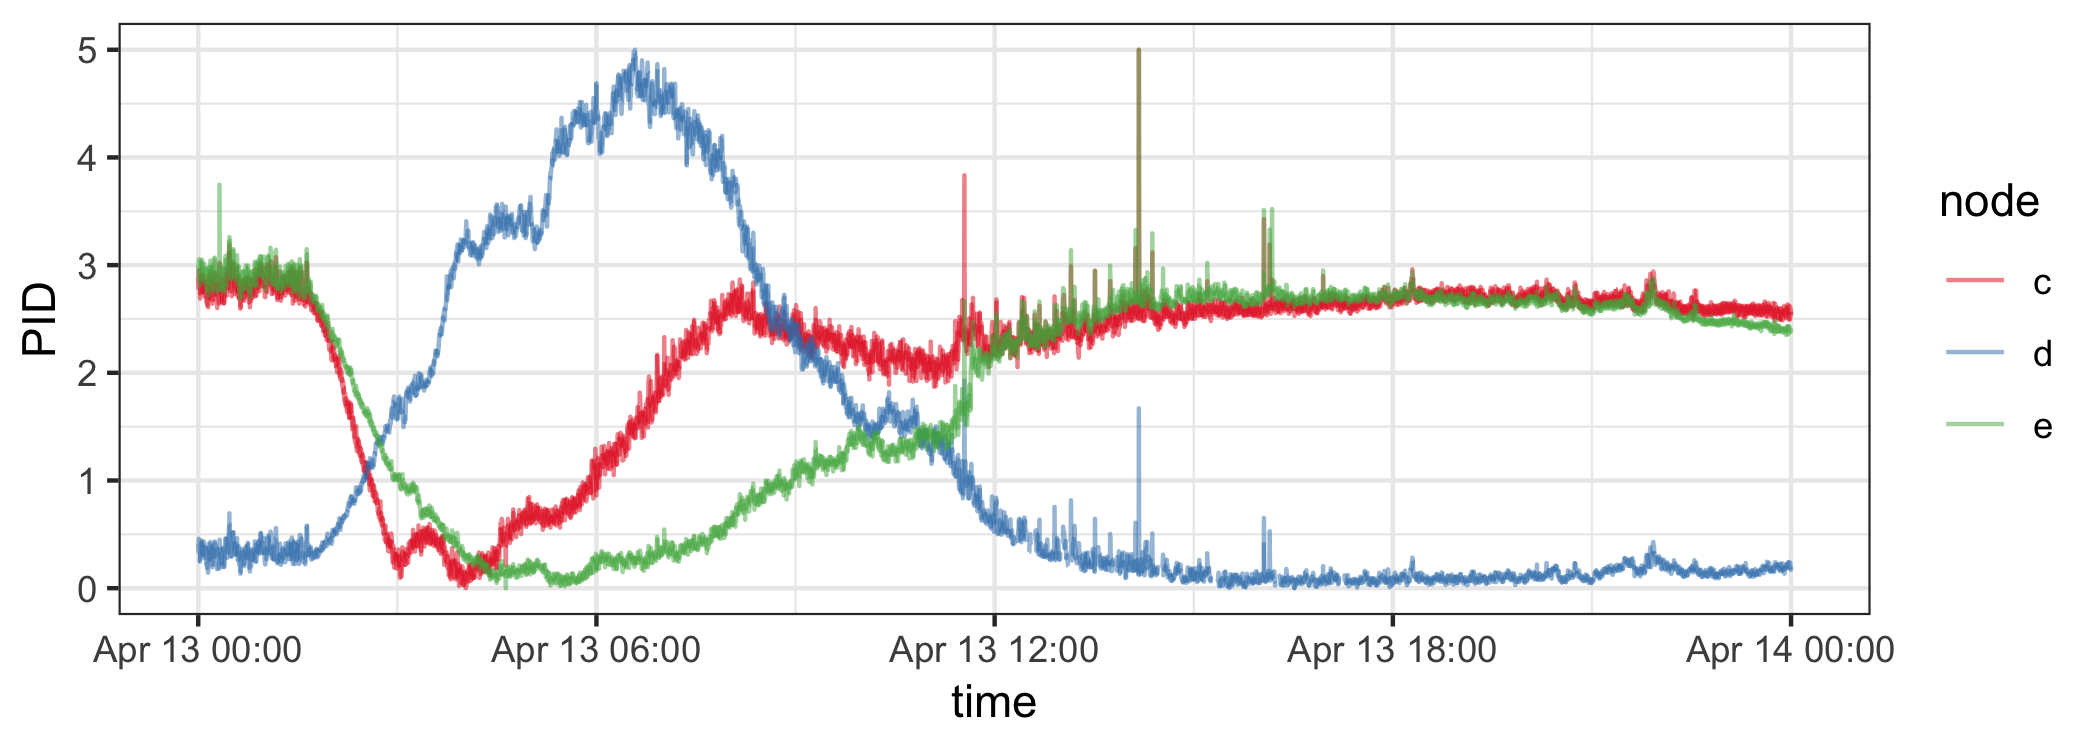
\includegraphics[width = \linewidth]{Figures/uncorrected_data.png}		
		\caption{Example of 3 co-located SPod PID sensor readings.}
		\label{fig:raw_spod}
	\end{figure}	

To tackle demixing problems, we introduce a scalable baseline estimation framework by building on \textit{$\ell_1$-trend filtering}, a relatively new nonparametric estimation framework. Our contributions are three-fold. 
\begin{itemize}
\item \cite{Kim2009} proposed using the check function as a possible extension of $\ell_1$-trend filtering but did not investigate it further. Here, we develop the basic $\ell_1$-quantile-trend-filtering framework and extend it to model multiple quantiles simultaneously with non-crossing constraints to ensure valid trend estimates. 
\item To reduce computation time and extend the method to long time series, we develop a parallelizable ADMM algorithm. 
\item Finally, we propose a modified criterion for performing model selection.
\end{itemize}

	In the rest of the paper, we detail our quantile trend filtering algorithms as well as how to choose the smoother parameter $\lambda$ (Section \ref{sec:methods}). We demonstrate through simulation studies that our proposed model provides better or comparable estimates of non-parametric quantile trends than existing methods (Section \ref{sec:simluation}). We further show that quantile trend filtering is a more effective method of drift removal for low-cost air quality sensors and results in improved signal classification compared to quantile smoothing splines (Section \ref{sec:application}). Finally, we discuss potential extensions of quantile trend filtering (Section \ref{sec:discussion}). 

%% ----------------------------------------------------------------------
%% Methods
%% ----------------------------------------------------------------------
\section{Baseline Trend Estimation}
\label{sec:methods}

%We review \textit{$\ell_1$-trend filtering} for estimating a mean trend before discussing how to adapt it to estimate a baseline trend. We then describe a new scalable algorithm for simultaneously computing multiple quantile trends over large times windows.

%% ----------------------------------------------------------------------
%% Background
%% ----------------------------------------------------------------------
\subsection{Background}

\cite{Kim2009} originally proposed \textit{$\ell_1$-trend filtering} to estimate trends with piecewise polynomial functions, assuming that the observed time series $\V{y}$ consists of a trend $\V{\theta}$ plus uncorrelated noise $\V{\varepsilon}$, namely $\V{y} = \V{\theta} + \V{\varepsilon}$. The estimated trend is the solution to the following convex optimization problem
\begin{eqnarray*}
\underset{\V{\theta}}{\text{minimize}}\; \frac{1}{2} \lVert \V{y} - \V{\theta} \rVert_2^2 + \lambda \lVert \Mn{D}{k+1}\V{\theta} \rVert_1,
\end{eqnarray*}
	where $\lambda$ is a nonnegative regularization parameter, and the matrix $\Mn{D}{k+1} \in \Real^{(n - k -1) \times n}$ is the discrete difference operator of order $k+1$. To understand the purpose of penalizing the size of $\Mn{D}{k+1}\V{\theta}$ consider the difference operator when $k = 0$.
	
	\begin{eqnarray*}
	\Mn{D}{1} & = & \begin{pmatrix}
	-1 & 1 & 0 & \cdots & 0 & 0 \\
	0 & -1 & 1 & \cdots & 0 & 0 \\
	\vdots & \vdots & \vdots & \ddots & \vdots & \vdots \\
	0 & 0 & 0 & \cdots & -1 & 1 \\
	\end{pmatrix}.
	\end{eqnarray*}
	
	Thus, $\lVert \Mn{D}{1}\V{\theta} \rVert_1 = \sum_{i=1}^{n-1} \lvert \theta_i - \theta_{i+1} \rvert$, which is known as total variation denoising penalty in one dimension in the signal processing literature \citep{Rudin1992} or the fused lasso penalty in the statistics literature \citep{Tibshirani2005}. The penalty term incentivizes solutions which are piecewise constant. For $k \geq 1$, the difference operator $\Mn{D}{k+1} \in \Real^{(n-k-1) \times n}$ is defined recursively as follows
	\begin{eqnarray*}
	\Mn{D}{k+1} & = & \Mn{D}{1}\Mn{D}{k}.
	\end{eqnarray*}
	Penalizing the 1-norm of the vector $\Mn{D}{k+1}\V{\theta}$ produces estimates of $\V{\theta}$ that are piecewise polynomials of order $k$.
	
%	$k+1$ fold composition of the discrete difference operator produces estimates that are piecewise polynomials of order $k$.

%\cite{Tib2014} later demonstrated empirically that the trend filtering estimates adapt to the local level of smoothness better than smoothing splines and also proved that with a judicious choice of tuning parameter the trend filtering estimate converges to the true underlying function at the minimax rate for functions whose $k$th derivative is of bounded variation. 
%	
%	Given observations $y(t)$ with $t=1,...,N$ and defining $y \in \Real^n$ such that $y_i = y(t)$, in the trend filtering problem, the trend, $\V{\theta} \in \Real^n$, is estimated by solving the following convex problem:
%	\begin{eqnarray}
%	\underset{\V{\theta}}{\arg\min}\; \frac{1}{2} \lVert y - \V{\theta} \rVert_2^2 + \lambda \lVert \Mn{D}{k+1}\V{\theta} \rVert_1,
%	\end{eqnarray}
%	where $y \in \Real^n$ is the vector of observations, $\lambda \geq 0$ is a regularization parameter, and the matrix $\Mn{D}{k+1} \in \Real^{(n - k -1) \times n}$ is the discrete difference operator of order $k+1$. To understand the purpose of penalizing $\Mn{D}{k+1}$ consider the difference operator when $k = 0$.
%	\begin{eqnarray*}
%	\Mn{D}{1} & = & \begin{pmatrix}
%
%	-1 & 1 & 0 & \cdots & 0 & 0 \\
%	0 & -1 & 1 & \cdots & 0 & 0 \\
%	\vdots & & & & & \\
%	0 & 0 & 0 & \cdots & -1 & 1 \\
%
%	\end{pmatrix}.
%	\end{eqnarray*}
%	Thus, $\lVert \Mn{D}{1}\V{\theta} \rVert_1 = \sum_{i=1}^{n-1} \lvert \theta_i - \theta_{i+1} \rvert$ which is just total variation denoising in one dimension. The penalty term incentivizes solutions which are piecewise constant. For $k \geq 1$, the difference operator $\Mn{D}{k+1} \in \Real^{(n-k-1) \times n}$ is defined recursively as follows
%	\begin{eqnarray*}
%	\Mn{D}{k+1} & = & \Mn{D}{1}\Mn{D}{k}.
%	\end{eqnarray*}
%	By penalizing the $k+1$ fold composition of the discrete difference operator, we obtain solutions which are piecewise polynomials of order $k$.
	
	\cite{Tib2014} proved that with a judicious choice of $\lambda$ the trend filtering estimate converges to the true underlying function at the minimax rate for functions whose $k$th derivative is of bounded variation and showed that trend filtering is both fast and locally adaptive when the time series consists of only the trend and random noise, which is illustrated in \Fig{tpn}. As noted earlier though in some applications, such as the air quality monitoring problem considered in this paper, the data contain a rapidly varying signal in addition to the slowly varying trend and noise. \Fig{tpspn} shows that standard trend filtering is not designed to distinguish between the slowly varying trend and the rapidly-varying signal, as the smooth component estimate $\V{\theta}$ is biased towards the peak of the transient component.
	
	To account for the presence of a transient component in the observed time series $\V{y}$, we propose quantile trend filtering \Fig{tpspn}. % as a more robust method for detrending in these situations \Fig{tpspn}. 
	To estimate the trend in the $\tau$\textsuperscript{th} quantile, we solve the convex optimization problem
	\begin{eqnarray}
	\label{eq:quantile_trend}
	\underset{\V{\theta}}{\text{minimize}}\; \rho_\tau(\V{y} - \V{\theta}) + \lambda \lVert \Mn{D}{k+1} \V{\theta} \rVert_1,
	\end{eqnarray}
	where $\rho_\tau(\V{r})$ is the check function
	\begin{eqnarray}
	\label{eq:check}
	\rho_{\tau}(\V{r}) & = & \sum_{i=1}^n \VE{r}{i}(1-\One(\VE{r}{i}<0)),
	\end{eqnarray}
	and $\One(A)$ is 1 if its input $A$ is true and 0 otherwise. 
		   	
	\begin{figure}
		\centering
		\subfloat[Slow Trend + Noise]{\label{fig:tpn}
		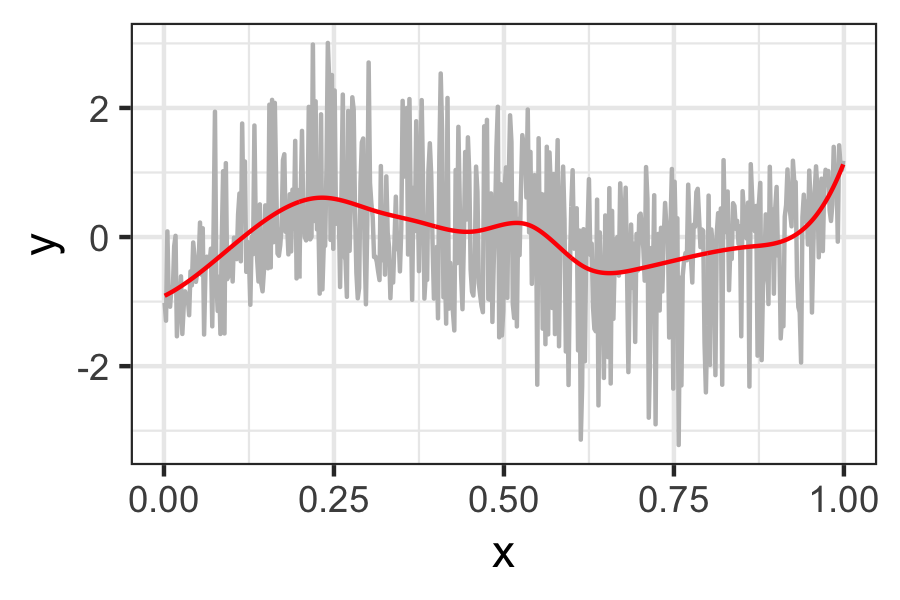
\includegraphics[width = 0.45\linewidth]{Figures/trend_filter_eg1.png}}
		\subfloat[Slow Trend + Spikes + Noise]{\label{fig:tpspn}
		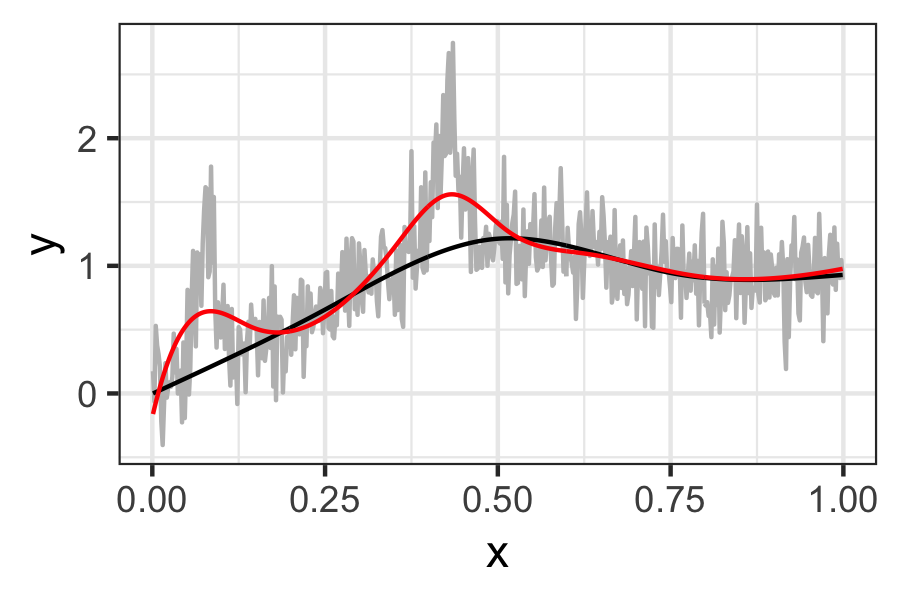
\includegraphics[width = 0.45\linewidth]{Figures/trend_filter_eg2.png}}
		\caption{Examples of trend filtering solutions (red) and 15\textsuperscript{th} quantile trending filtering solution (blue). Standard trend filtering performs well in the no-signal case (right) but struggles to distinguish between the slowly varying trend and the rapidly-varying signal (left). The quantile trend is not affected by the signal and provides an estimate of the baseline.}
	\end{figure}
	Note that we do not explicitly model $\V{s}$. Rather, we focus on estimating $\V{\theta}$. We then estimate $\V{s} + \V{\varepsilon}$ as the difference $\V{y} - \V{\theta}$.

	Before elaborating on how we compute our proposed $\ell_1$-quantile trend filtering estimator, we discuss similarities and differences between our proposed estimator and existing baseline estimators.

%% ----------------------------------------------------------------------
%% Relationship to Prior Work
%% ----------------------------------------------------------------------
\subsubsection{Relationship to Prior Work}

	In this application, as well as those described in \cite{Ning2014}, \cite{marandi2015qualitative}, and \cite{pettersson2013algorithm}, the goal is to estimate the trend in the baseline not the mean. We can define the trend in the baseline as the trend in a low quantile of the data. A variety of methods for estimating quantile trends have already been proposed. \cite{Koenker1978} were the first to propose substituting the sum-of-squares term with the check function  \Eqn{check} to estimate a conditional quantile instead of the conditional mean. Later, \cite{KoenkerNgPortnoy1994} proposed quantile trend filtering with $k = 2$ producing quantile trends that are piecewise linear, but they did not consider extensions to higher order differences. Rather than using the $\ell_1$-norm to penalize the discrete differences, \cite{nychka1995nonparametric} used the smoothing spline penalty based on the square of the $\ell_2$-norm: 
	
	\begin{equation*}
	\label{eq:smoothingspline}
	\sum_{i=1}^n\rho_{\tau}(y(t_i) - \theta(t_i)) + \lambda\int \theta''(t)^2 dt, 
 	\end{equation*}	
	where $\theta(t)$ is a smooth function of time and $\lambda$ is a tuning parameter that controls the degree of smoothing. \cite{Oh2011} proposed an algorithm for solving the quantile smoothing spline problem by approximating the check function with a differentiable function. \cite{Racine2017} take a different approach and constrain the response to follow a smooth location scale model of the form $y(t) = a(t) + b(t)\epsilon_i$ and estimate the $\tau$\textsuperscript{th} conditional quantile using a kernel estimator and local linear approach. \Halley{Eric}{What are $a(t), b(t)$, and $\epsilon_i$?}


%% ----------------------------------------------------------------------
%% Quantile Trend Filtering
%% ----------------------------------------------------------------------
\subsection{Quantile Trend Filtering}

	We combine the ideas of quantile regression and trend filtering. For a single quantile level $\tau$, the quantile trend filtering problem is given in \Eqn{quantile_trend}. As with classic quantile regression, the quantile trend filtering problem is a linear program which can be solved by a number of methods. In many cases, including ours, we are interested in estimating multiple quantiles simultaneously. We also want to ensure that our quantile estimates are valid by enforcing the constraint that if $\tau_2 > \tau_1$ then $Q(\tau_2) \ge Q(\tau_1)$ where $Q$ is the quantile function of $\V{y}$. Given quantiles $\tau_1 < \tau_2 < \ldots < \tau_J$, the optimization problem becomes 
	\begin{eqnarray*}
	\label{eq:noncross_trend}
%	&&\underset{\V{\theta}_1, \ldots, \V{\theta}_J}{\text{minimize}}\; \sum_{j=1}^J \left [\rho_{\tau_j}(\V{y} - \V{\theta}_{j}) + 
%	\lambda_j \lVert \Mn{D}{k+1} \V{\theta}_j \rVert_1 \right ] \\	
	&&\underset{\M{\Theta} \in \mathcal{C}}{\text{minimize}}\; \sum_{j=1}^J \left [\rho_{\tau_j}(\V{y} - \V{\theta}_{j}) + 
	\lambda \lVert \Mn{D}{k+1} \V{\theta}_j \rVert_1 \right ] \\
%	&&\text{subject to: }\; \V{\theta}_1 \leq \V{\theta}_2 \leq \ldots \leq \V{\theta}_J	
%	\theta_{1}(t) \le \theta_{2}(t) \le \ldots \le \theta_{J}(t) \text{ for all } t, \nonumber
	\end{eqnarray*}
	where $\M{\Theta} = \begin{pmatrix} \V{\theta}_1 & \V{\theta}_2 & \cdots & \V{\theta}_J \end{pmatrix} \in \Real^{n \times J}$ is a matrix whose $j$th column corresponds to the $j$th quantile signal $\V{\theta}_j$ and the set $\mathcal{C} = \{\M{\Theta} \in \Real^{n \times J}: \ME{\theta}{ij} \leq \ME{\theta}{ij'} \;\text{for $j \leq j'$}\}$ encodes the non-crossing quantile constraints. The additional constraints are linear in the parameters, so the non-crossing quantile trends can still be estimated by a number of available solvers. In the rest of this paper, we report numerical results using the commercial solver Gurobi \citep{gurobi} and its R package implementation. However, we could easily substitute a free solver such as the Rglpk package by \cite{rglpk}. 

%% ----------------------------------------------------------------------
%% ADMM for Big Data
%% ----------------------------------------------------------------------
\subsection{ADMM for Big Data}
	
The number of parameters to be estimated in this problem is equal to the number of observations multiplied by the number of quantiles of interest. As the size of the data and the number of quantiles grows, all solvers will eventually break \Halley{Eric}{Can we be more specific about what we mean when we say ``break?"}. To our knowledge, no one has addressed the problem of finding smooth quantile trends of series that are too large to be processed simultaneously. We propose a divide-and-conquer approach via an ADMM algorithm for solving large problems in a piecewise fashion. The ADMM algorithm \citep{gabay1975dual, glowinski1975approximation} is  described in greater detail by \cite{boyd2011distributed}, but we briefly review how it can be used to iteratively solve the following equality constrained optimization problem.
\begin{equation}
\label{eq:split_objective}
\begin{split}
&\text{minimize} \; f(\V{\theta}) + g(\Vtilde{\theta}) \\
&\text{subject to} \; \M{A}\V{\theta} + \M{B}\Vtilde{\theta} = \V{c}.
\end{split}
\end{equation}
Recall that finding the minimizer to an equality constrained optimization problem is equivalent to the identifying the saddle point of the Lagrangian function associated with the problem \Eqn{split_objective}. ADMM seeks the saddle point of a related function called the augmented Lagrangian,
%The Lagrangian for the ALM problem
\begin{eqnarray*}
\mathcal{L}_{\gamma}(\V{\theta},\Vtilde{\theta},\V{\omega}) & = & f(\V{\theta}) + g(\Vtilde{\theta}) + \langle \V{\omega}, \V{c} - \M{A}\V{\theta} - \M{B}\Vtilde{\theta} \rangle
+ \frac{\gamma}{2} \lVert \V{c} - \M{A}\V{\theta} - \M{B}\Vtilde{\theta} \rVert_2^2,
\end{eqnarray*}
where the dual variable $\V{\omega}$ is a vector of Lagrange multipliers and $\gamma$ is a nonnegative tuning parameter. When $\gamma = 0$, the augmented Lagrangian coincides with the ordinary Lagrangian.

ADMM minimizes the augmented Lagrangian one block of variables at a time before updating the dual variable $\V{\omega}$. This yields the following sequence of updates at the $m+1$th ADMM iteration
\begin{equation}
\label{eq:admm_updates}
\begin{split}
\V{\theta}_{m+1} & \amp = \amp \underset{\V{\theta}}{\arg\min}\; \mathcal{L}_\gamma(\V{\theta},\Vtilde{\theta}_{m}, \V{\omega}_{m}) \\
\Vtilde{\theta}_{m+1} & \amp = \amp \underset{\Vtilde{\theta}}{\arg\min}\; \mathcal{L}_\gamma(\V{\theta}_{m+1},\Vtilde{\theta}, \V{\omega}_{m}) \\
\V{\omega}_{m+1} & \amp = \amp \V{\omega}_{m} + \gamma(\V{c} - \M{A}\V{\theta}_{m+1} - \M{B}\Vtilde{\theta}_{m+1}).
\end{split}
\end{equation}
	
	
	
	Let $\mathcal{I}$ denote a subset of the indices $\{1, \ldots, n\}$ and $\V{y}_\mathcal{I} \in \Real^{\lvert I \rvert}$ denote the subvector obtained by stacking on top of each other the elements $\VE{y}{i}$ for $i \in \mathcal{I}$ in their canonical ordering.	
	We apply the consensus ADMM algorithm to the quantile regression trend filtering problem given in \Eqn{quantile_trend}, by dividing our observed series $\VE{y}{i}$ with $i = 1, \ldots, n$ into overlapping $W$ windows of observations $\Vn{y}{w} = \V{y}_{\mathcal{I}_w}$ where $\mathcal{I}_w$ is the set of integers from $l_w$ to $u_w$ inclusive, namely $\mathcal{I}_w = \{l_w, l_w + 1, \ldots, u_w -1, u_w\}$ where 
\begin{eqnarray*}
1 = l_{1} < l_{2} < u_{1} < l_{3} < u_{2} < l_{4} < u_{3} < \cdots < u_{W} = n.
\end{eqnarray*}
\Fig{windows} shows an example of 1200 observations being mapped into three equally sized overlapping windows of observations. 
		
%	\begin{align*}
%	y_1(t) = y(t) & \mbox{~~if~~} 1 \le t \le u_{1}\\
%	y_2(t) = y(t) & \mbox{~~if~~} l_{2} \le t \le u_{2} \\
%	\vdots & \\
%	y_M(t) = y(t) & \mbox{~~if~~} l_{M} \le t \le  n,
%	\end{align*}
%
%	 with boundaries $1 < l_{2} < u_{1} < l_{3} < u_{2} < l_{4} < u_{3} < ...< n$. 
%	 Given quantiles $\tau_1 < \cdots < \tau_J$, we define $\theta_{j,m}(t)$ as the value of the $\tau_j$\textsuperscript{th} quantile trend in window $m$ at time $t$. In order to constrain the overlapping sections to be equal, we define a consensus variable	 
Given quantiles $\tau_1 < \cdots < \tau_J$, we introduce dummy variables $\Vn{\theta}{w}_{j} \in \Real^{\lvert \mathcal{I}_w \rvert}$ as the value of the $\tau_j$\textsuperscript{th} quantile trend in window $w$. We then ``stitch" together the $W$ quantile trend estimates into consensus over the overlapping regions by introducing the constraint $\VnE{\theta}{w}{ij} = \VE{\theta}{i + l_w - 1,j}$ for $i = 1, \ldots, u_w - l_w + 1$ and for all $j$. Let $\Mn{\Theta}{w}$ be the matrix whose $j$th column is $\Vn{\theta}{w}$. Then we can write these constraints more compactly as $\Mn{\Theta}{w} = \Mn{U}{w}\M{\Theta}$, where $\Mn{U}{w} \in \{0, 1\}^{\lvert \mathcal{I}_w \rvert \times n}$ is a matrix that selects rows of $\M{\Theta}$ corresponding to the $w$th window, namely
\begin{eqnarray*}
\Mn{U}{w} & = & \begin{pmatrix}
\V{e}_{l_w}\Tra \\
\vdots \\
\V{e}_{u_w}\Tra
\end{pmatrix},
\end{eqnarray*}
where $\V{e}_i \in \Real^{n}$ denotes the $i$th standard basis vector. Furthermore, let $\iota_{\mathcal{C}}$ denote the indicator function of the non-crossing quantile constraint, namely $\iota_{\mathcal{C}}(\M{\Theta})$ is zero if $\M{\Theta} \in \mathcal{C}$ and infinity otherwise.
	 
	Our windowed quantile trend optimization problem can then be written as 
	 \begin{equation}
		 \label{eq:quantile_windows}
		 \begin{split}
		 &\text{minimize}\; \sum_{w=1}^W \left \{\sum_{j=1}^J \left [\rho_{\tau_j}(\Vn{y}{w} - \Vn{\theta}{w}_{j}) + 
		 \lambda \lVert \Mn{D}{k+1} \Vn{\theta}{w}_{j} \rVert_1 \right ] + \iota_\mathcal{C}(\Mn{\Theta}{w}) \right\}\\
		 &\text{subject to} \qquad \Mn{\Theta}{w} = \Mn{U}{w}\M{\Theta} \;\; \text{ for } w = 1, \ldots, W.
		 \end{split}
	 \end{equation}	 
	 
	 	 Let $\Mn{\Omega}{w}$ denote the Lagrange multiplier matrix for the $w$th consensus constraint, namely $\Mn{\theta}{w} = \Mn{U}{w}\M{\theta}$, and let $\Vn{\omega}{w}_{j}$ denote its $j$th column.
%		 
%		  $\V{\omega}_{m}_{j}$ denote Lagrange multipliers for the constraint $\Vn{\theta}{w}_j = \Mn{U}{m}\V{\theta}_j$, $\Mn{\Omega}{m}$ denote the matrix whose $j$th column is $\V{\omega}_{m}_j$, and penalty parameter $\gamma > 0$, 
		  
		  The augmented Lagrangian is given by
	 \begin{eqnarray*}
	 \mathcal{L}(\M{\Theta}, \{\Mn{\Theta}{w}\}, \{\Mn{\Omega}{w}\}) & = & \sum_{w=1}^W \mathcal{L}_w(\M{\Theta}, \Mn{\Theta}{w}, \Mn{\Omega}{w}),
\end{eqnarray*}
where
\begin{eqnarray*}
 \mathcal{L}_w(\M{\Theta}, \Mn{\Theta}{w}, \Mn{\Omega}{w}) & = & \sum_{j=1}^J \biggl [\rho_{\tau_j}(\Vn{y}{w} - \Vn{\theta}{w}_j)+\lambda \lVert \Mn{D}{k+1}\Vn{\theta}{w}_j\rVert_1 \\
	 && + \; (\Vn{\theta}{w}_j - \Mn{U}{w}\V{\theta}_{j})\Tra\Vn{\omega}{w}_{j} + 
	 \frac{\gamma}{2}\lVert \Vn{\theta}{w}_j - \Mn{U}{w}\V{\theta}_{j}\rVert_2^2 \biggr ] + \iota_\mathcal{C}(\Mn{\Theta}{w}),
	 \end{eqnarray*}
	 where $\gamma$ is a positive penalty parameter. 

The ADMM algorithm alternates between updating the consensus variable $\M{\Theta}$, the window variables $\{\Mn{\Theta}{w}\}$, and the Lagrange multipliers $\{\Mn{\Omega}{w}\}$. 
At the $m+1$th iteration, we perform the following sequence of updates	 

\begin{eqnarray*}
	\M{\Theta}_{m+1} & = & \underset{\M{\Theta}}{\arg\min}\; \mathcal{L}(\M{\Theta}, \{\Mn{\Theta}{w}_m\}, \{\Mn{\Omega}{w}_m\}) \\
	\Mn{\Theta}{w}_{m+1} & = & \underset{\{\Mn{\Theta}{w}\}}{\arg\min}\; \mathcal{L}(\M{\Theta}_{m+1}, \{\Mn{\Theta}{w}\}, \{\Mn{\Omega}{w}_m\}) \\
\end{eqnarray*}

{\bf Updating $\M{\Theta}$: } Some algebra shows that updating the consensus variable step is computed as follows.

\begin{eqnarray}
\label{eq:update_consensus}
\ME{\theta}{ij}	 &=& \begin{cases} 
			 \frac{1}{2}\left (\MnE{\theta}{w-1}{ij} - \gamma\Inv \MnE{\omega}{w-1}{ij} \right)
			 + 
			 \frac{1}{2} \left (\MnE{\theta}{w}{ij} - \gamma\Inv \MnE{\omega}{w}{ij} \right)
			  & \mbox{if~~} l_{w} \le i \le u_{w-1},  \\
			 \MnE{\theta}{w}{ij} & \mbox{if~~} u_{w-1} < i \le l_{w+1}  \\
			 \frac{1}{2} \left ( \MnE{\theta}{w}{ij} - \gamma\Inv \MnE{\omega}{w}{ij}\right )
			 + 
			 \frac{1}{2}	\left ( \MnE{\theta}{w+1}{ij} - \gamma\Inv \MnE{\omega}{w+1}{ij} \right )
			 & \mbox{if~~} l_{m+1} < i \le u_{m}  
			 \end{cases},
\end{eqnarray}	

The consensus update \Eqn{update_consensus} is rather intuitive. We essentially average the trend estimates in overlapping sections of the windows, subject to some adjustment by the Lagrange multipliers, and leave the trend estimates in non-overlapping sections of the windows untouched. 
%This appears like we need to invert an underdetermined linear system, but we're actually just picking off the relevant entries.
For notational ease, we write the consensus update \Eqn{update_consensus} compactly as $\M{\Theta} = \psi(\{\Mn{\Theta}{w}\},\{\Mn{\Omega}{w}\})$.

{\bf Updating $\{\Mn{\Theta}{w}\}$: } We then estimate the trend separately in each window, which can be done in parallel, while constraining the overlapping pieces of the trends to be equal as outlined in \Alg{admm}. The use of the Augmented Lagrangian converts the problem from a linear program into a quadratic program. The \texttt{gurobi} R package \citep{gurobi} can solve quadratic programs in addition to linear programs, but we can also use the free R package \texttt{quadprog} \citep{quadprog}. 
	 
%	 \begin{eqnarray*}
%	\M{A}r{\theta}_{j, m}	&=&  g(\theta_{j, m-1}, \theta_{j,m}, \theta_{j,m+1}) \\
%	\M{A}r{\theta}_{j, m}(t)	 &=& \begin{cases} 
%			 \frac{\theta_{j,m-1}(t)+\theta_{j,m}(t)}{2} & \mbox{if~~} l_{m} \le t \le u_{m-1}  \\
%			 \theta_{j,m}(t) & \mbox{if~~} u_{m-1} \le t \le l_{m+1}  \\
%			 \frac{\theta_{j,m}(t)+\theta_{j,m+1}(t)}{2} & \mbox{if~~} l_{m+1} \le t \le u_{m}  
%			 \end{cases},
%	\end{eqnarray*}
%	 
%	 \begin{align*}
%	\M{A}r{\theta}_{j, m}	=&  g(\theta_{j, m-1}, \theta_{j,m}, \theta_{j,m+1}) \\
%	\M{A}r{\theta}_{j, m}(t)	 =& \begin{cases} 
%			 \frac{\theta_{j,m-1}(t)+\theta_{j,m}(t)}{2} & \mbox{if~~} l_{m} \le t \le u_{m-1}  \\
%			 \theta_{j,m}(t) & \mbox{if~~} u_{m-1} \le t \le l_{m+1}  \\
%			 \frac{\theta_{j,m}(t)+\theta_{j,m+1}(t)}{2} & \mbox{if~~} l_{m+1} \le t \le u_{m}  
%			 \end{cases},
%	\end{align*}
%	defining $\theta_{j,M+1} = \theta_{j,M}$ and $\theta_{j,0} = \theta_{j,1}$. Our windowed quantile trend optimization problem can then be written as 
%	 \begin{align*}
%		 \label{eq:quantile_windows}
%		 &\underset{\theta_{1,m}, \ldots, \theta_{J,m}}{\text{minimize}}\; \sum_{m=1}^M\sum_{j=1}^J \left [\rho_{\tau_j}(\Vn{y}{m} - \theta_{j,m}) + 
%		 \lambda_j \lVert \Mn{D}{k+1} \theta_{j,m} \rVert_1 \right ] \\
%		 &\text{subject to: }\; \\
%		 &\qquad \theta_{1,m}(t) \le \theta_{2,m}(t) \le \ldots \le \theta_{J,m}(t) \text{ for all } m,t \\
%		 &\qquad \theta_{j,m}(t) = \M{A}r{\theta}_{j,m}(t) \text{ for all } j, m, t
%	 \end{align*}
%	 Defining Lagrange multipliers $\omega_{j,m}$, and penalty parameter $\gamma > 0$, the augmented Lagrangian for finding the trends in window $m$ is
%	 \begin{equation*}
%	 \mathcal{L}(\theta_{j,m}, \M{A}r{\theta}_{j,m}, \omega_{j,m}) = \sum_{j=1}^J\rho_{\tau_j}(\Vn{y}{m} - \theta_{j,m})+\lambda \lVert \Mn{D}{k+1}\theta_{j,m}\rVert_1 +  \omega_{j,m}\Tra(\theta_{j,m} - \M{A}r{\theta}_{j,m}) + 
%	 \frac{\gamma}{2}||\theta_{j,m} - \M{A}r{\theta}_{j,m}||_2^2
%	 \end{equation*}
%	 We then estimate the trend separately in each window, which can be done in parallel, while constraining the overlapping pieces of the trends to be equal as outlined in Algorithm 1. The use of the Augmented Lagrangian converts the problem from a linear program into a quadratic program. The \texttt{gurobi} R package \citep{gurobi} can solve quadratic programs in addition to linear programs, but we can also use the free R package \texttt{quadprog} \citep{quadprog}. 
%	 
	\begin{figure}[!t] 
		\centering
		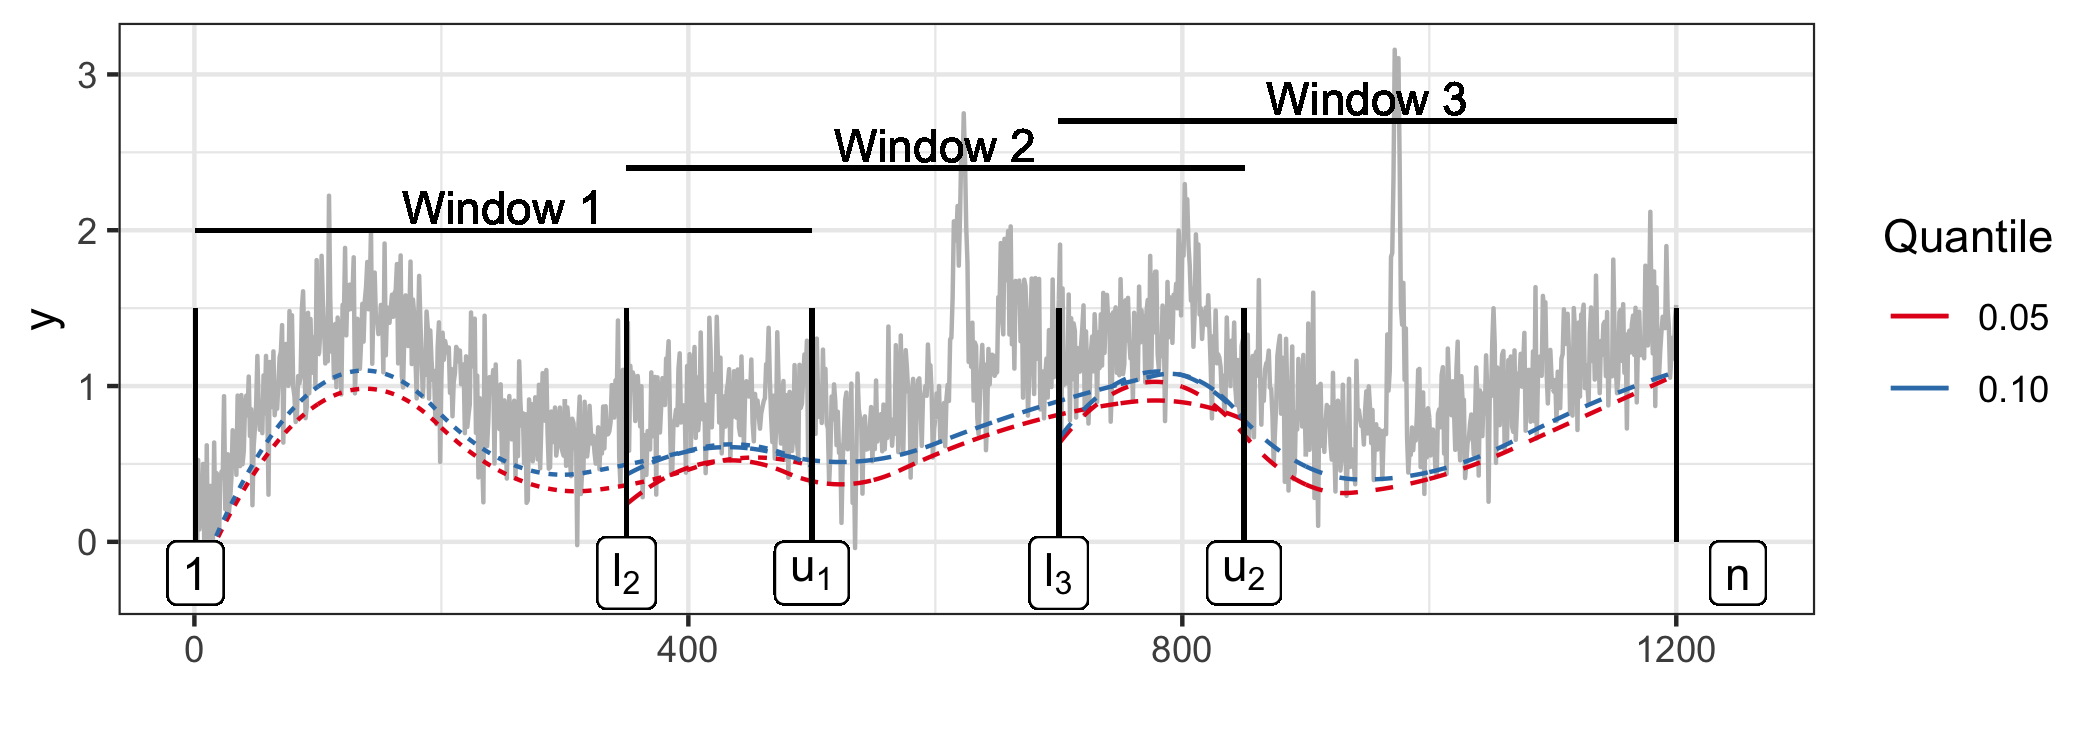
\includegraphics[width = 0.8\linewidth]{Figures/overlapping_windows.png}
		\caption{Window boundaries and trends fit separately in each window.}		
		\label{fig:windows}
	\end{figure}

	\begin{algorithm}
		\caption{ADMM algorithm for quantile trend filtering with windows}\label{alg:admm}
		\begin{algorithmic}		
			\State Define $\M{D} = \Mn{D}{k+1}$. 
			\State \textbf{initialize:}
			\For{$w = 1, \ldots, W$}
			\State $\Mn{\Theta}{w}_0 \gets \underset{\Mn{\Theta}{w} \in \mathcal{C}}{\arg \min}\; 			
			 \sum_{j=1}^J\rho_{\tau_j}(\Vn{y}{w} - \Vn{\theta}{w}_{j})+\lambda \lVert \M{D}\Vn{\theta}{w}_{j}\rVert_1$
%				 $\Vn{\theta}{0}_{j,m} \gets \arg \min \sum_{j=1}^J\rho_{\tau_j}(\Vn{y}{w} - \V{\theta}_{j,m})+\lambda \lVert \M{D}\V{\theta}_{j,m}\rVert_1$ subject to $\theta_{1,m}(t) < \ldots<\theta_{J,m}(t)$ for all $t$. \\		
			\State $\Mn{\Omega}{w}_0 \gets \M{0}$
			\EndFor
%			 	 $\Vn{\omega}{0}_{j,m} \gets \V{0}$	
			\State $m \gets 0$
			\Repeat{}
			\State $\M{\Theta}_{m+1} \gets \psi(\{\Mn{\Theta}{w}_m\}, \{\Mn{\Omega}{w}_m\})$
			\For{$w = 1, \ldots, W$}			
			\State $\Mn{\Theta}{w}_{m+1} \gets \underset{\Mn{\Theta}{w}}{\arg\min}\; \mathcal{L}_w(\M{\Theta}_{m+1}, \Mn{\Theta}{w}, \Mn{\Omega}{w}_{m})$
			\State 
			$\Mn{\Omega}{w}_{m+1} \gets \Mn{\Omega}{w}_m + \gamma(\Mn{\Theta}{w}_{m+1} - \Mn{U}{w}\M{\Theta}_{m+1})$			
			\EndFor
			\State $m \gets m + 1$
%			\State  					
%			$\M{A}r{\theta}_{j,m}^{(q)} \gets g(\theta_{j, m-1}^{(q-1)}, \theta_{j,m}^{(q-1)}, \theta_{j,m+1}^{(q-1)})$
%			\State 
%			$\omega_{j,m}^{(q)} \gets \omega_{j,m}^{(q-1)} + \gamma(\theta_{j,m}^{(q-1)} - \M{A}r{\theta}_{j,m}^{(q)})$			
%			\State
%				$\theta_{j,m}^{(q)} \gets \arg\min \mathcal{L}(\theta_{j,m}, \M{A}r{\theta}_{j,m}^{(q-1)}, \omega_{j,m}^{(q-1)})$			
%			 subject to $\theta_{1,m}(t) < \ldots<\theta_{J,m}(t)$ for all $t$.
			\Until {convergence}
			\State \textbf{return} $\M{\Theta}_m$
%			\State \textbf{return} Non-overlapping sequence of $\M{A}r{\theta}_{j,m}^{(q)}$ for all $j$, $m$.			
		\end{algorithmic}
	\end{algorithm}

	To terminate our algorithm, we use the stopping criteria described by \cite{boyd2011distributed}. The criteria are based on the primal and dual residuals, which represent the residuals for primal and dual feasibility, respectively. The primal residual at the $m$th iteration, 
%	\begin{eqnarray*}
%	r_p^{(q)} & = & \sqrt{\sum_{m=1}^M\sum_{j=1}^J\lVert\theta_{j,m}^{(q)} - \M{A}r{\theta}_{j,m}^{(q)}\rVert_2^2},
%	\end{eqnarray*}
	\begin{eqnarray*}
	r_{\text{primal}}^{m} & = & \sqrt{\sum_{w=1}^W\lVert\Mn{\Theta}{w}_{m} - \M{\Theta}_m\rVert_{\text{F}}^2},
	\end{eqnarray*}
	represents the difference between the trend values in the windows and the consensus trend value. The dual residual at the $m$th iteration,
%	\begin{eqnarray*}
%	r_d^{(q)} & = & \gamma\sqrt{\sum_{m=1}^M \sum_{j=1}^J\lVert\M{A}r{\theta}_{j,m}^{(q)} - \M{A}r{\theta}_{j,m}^{(q-1)}\rVert_2^2},
%	\end{eqnarray*}
	\begin{eqnarray*}
	r_{\text{dual}}^{m} & = & \gamma\sqrt{\sum_{w=1}^W \lVert\M{\Theta}_m - \M{\Theta}_{m-1}\rVert_{\text{F}}^2},
	\end{eqnarray*}
	represents the change in the consensus variable from one iterate to the next. The algorithm is stopped when 
%	\begin{eqnarray*}
%		r_p^{(q)} & < &\epsilon_{\text{abs}}\sqrt{nJ} + \epsilon_{\text{rel}}\underset{w}{\max}\left[\max 
%		\left(\sqrt{\sum_{j=1}^J \lVert\theta_{j,m}^{(q)}\rVert_2^2}, \sqrt{\sum_{j=1}^J \lVert \M{A}r{\theta}_{j,m}^{(q)} \rVert_2^2} \right )\right]\\
%		r_d^{(q)} & < & \epsilon_{\text{abs}}\sqrt{nJ} + \epsilon_{\text{rel}}\sqrt{\sum_{m=1}^M\sum_{j=1}^J\lVert \omega_{j,m}^{(q)}\rVert_2^2}
%	\end{eqnarray*}
	\begin{eqnarray*}
		r_{\text{primal}}^{m} & < &\epsilon_{\text{abs}}\sqrt{nJ} + \epsilon_{\text{rel}}\,\underset{w}{\max} \left[\max 
		\left\{\lVert\Mn{\Theta}{w}_m \rVert_{\text{F}}, \lVert \M{\Theta}_{m} \rVert_{\text{F}} \right\}\right] \\%\lVert \M{\Theta}_{k} \rVert_{\text{F}}} \right )\right]\\
		r_{\text{dual}}^{m} & < & \epsilon_{\text{abs}}\sqrt{nJ} + \epsilon_{\text{rel}}\,\sqrt{\sum_{w=1}^W
		\lVert \Mn{\Omega}{w}_m \rVert_{\text{F}}^2}.
	\end{eqnarray*}	

	
	\begin{figure}
		\centering
		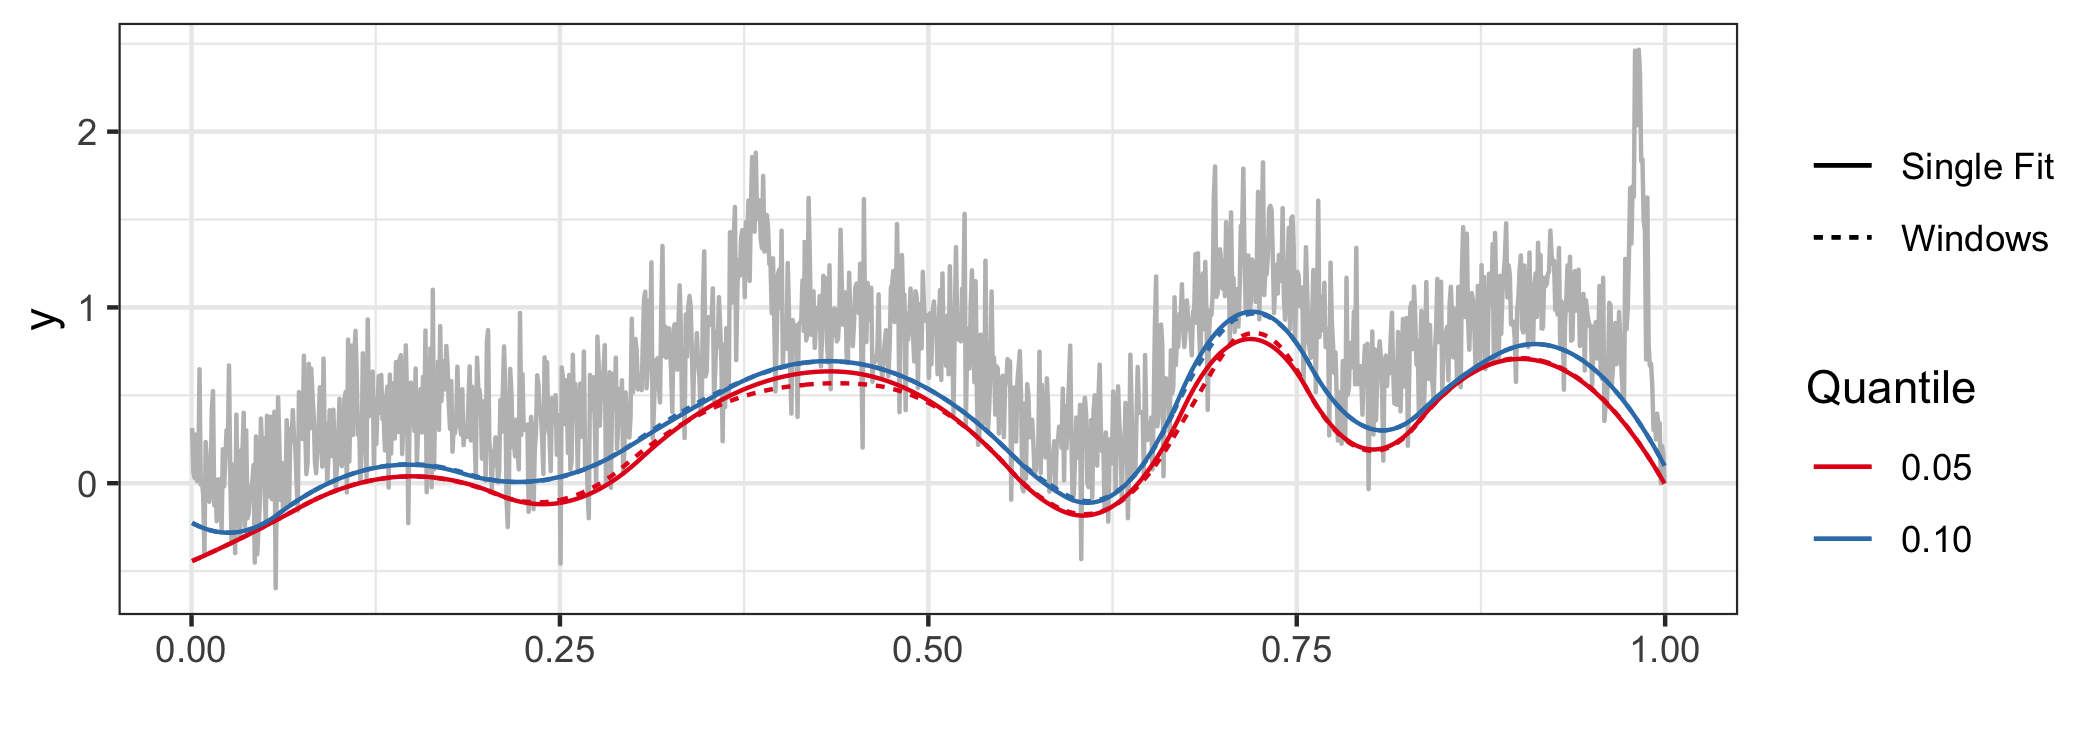
\includegraphics[width = 0.8\linewidth]{Figures/admm_windows.png}
		\caption{Trend fit with our ADMM algorithm with 3 windows which converged in 7 iterations compared to trend from simultaneous fit.}
	\end{figure}

	Timing experiments illustrate the advantages of using our ADMM algorithm when the trend can be estimated with a single window. For each data size, $n$, 25 datasets were simulated using the peaks simulation design described below. Trends for three quantiles were fit simultaneously: 0.05, 0.1, and 0.15 using $\lambda = n/5$. We use from one to four windows for each data size with an overlap of 500. The windows algorithm was run until the stopping criteria were met using $\epsilon_{abs} = 0.01$ and $\epsilon_{rel} = 0.001$. \Fig{timing} shows that using 4 windows instead of one on data sizes of 55000 provides a factor of 3 decrease in computation time. The timing experiments were conducted on an Intel Xeon based Linux cluster using two processor cores.   

	
	\begin{figure}[!t] 
		\centering
		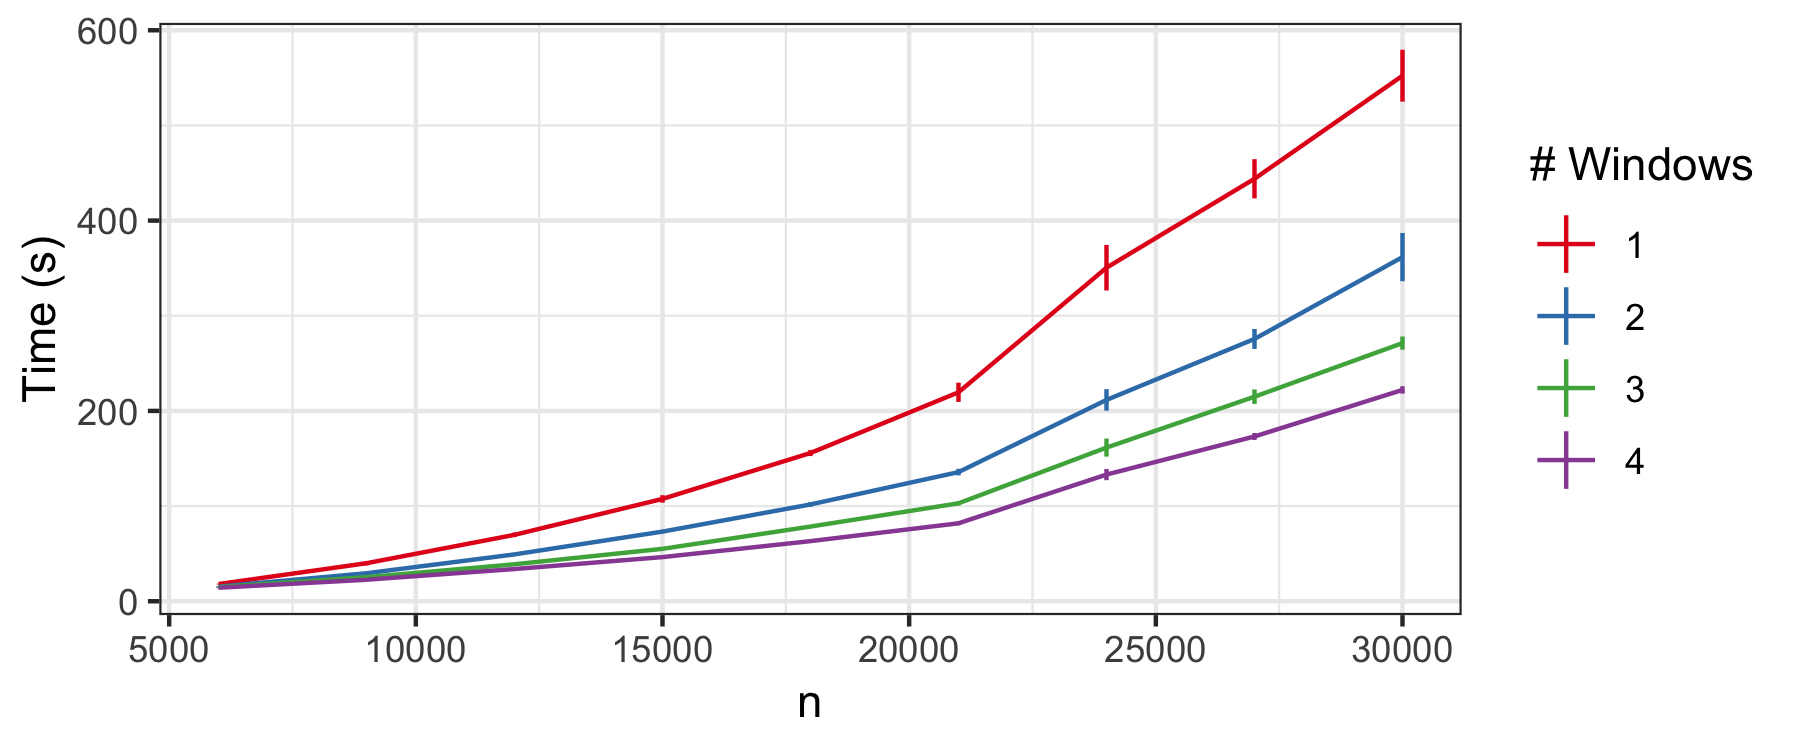
\includegraphics[width = 0.7\linewidth]{Figures/Fig_timing_experiment.png}
		\caption{Timing experiments comparing quantile trend filtering with varying numbers of windows by data size.}
		\label{fig:timing}
	\end{figure}

%% ----------------------------------------------------------------------
%% Computational Complexity and Convergence
%% ----------------------------------------------------------------------
\subsection{Computational Complexity and Convergence}

\Eric{Eric}{Add computational complexity of quadratic program and discuss the savings compared with solving a single large LP}.

\Alg{admm} has the following convergence guarantees.

\begin{proposition}
\label{prop:convergence}
Let $\{\{\Mn{\Theta}{w}_m\}, \M{\Theta}_m\}$ denote the $m$th collection of iterates generated by \Alg{admm}. Then (i) 
$\lVert \Mn{\Theta}{w}_m - \Mn{U}{w}\M{\Theta}_m \rVert_{\text{F}} \rightarrow 0$ and (ii) $p_m \rightarrow p^\star$, where $p^\star$ is the optimal objective function value of 
\Eqn{quantile_windows} and $p_m$ is the objective function value of \Eqn{quantile_windows} evaluated at $\{\{\Mn{\Theta}{w}_m\}, \M{\Theta}_m\}$.
\end{proposition}

The proof of \Prop{convergence} is a straightforward application of the convergence result presented in Section 3.2 of \cite{boyd2011distributed}.

%% ----------------------------------------------------------------------
%% Model Selection
%% ----------------------------------------------------------------------
	\section{Model Selection}
	\label{sec:lambda_choice}

	An important practical issue in baseline estimation is the choice of regularization parameter $\lambda$, which controls the degree of smoothness in $\V{\theta}$. In this section, we introduce four methods for choosing $\lambda$. The first is a validation based approach; the latter three are based on information criteria.

\subsection{Validation}	
	Our method can easily handle missing data by defining the check loss function to output 0 for missing values. %We also explore three information criteria.  
	Specifically, we use the following modified function $\tilde{\rho}_\tau$ in place of the $\rho_\tau$ function given in \Eqn{check}
	\begin{eqnarray}
	\label{eq:modcheck}
	\tilde{\rho}_{\tau}(\V{r}) & = & \sum_{i \not\in \mathcal{V}} \VE{r}{i}(1-\One(\VE{r}{i}<0)),
	\end{eqnarray}
	where $\mathcal{V}$ is a held-out validation subset of $\{1, \ldots, n\}$ and solve the problem
	
	\begin{eqnarray}
	\label{eq:validate}
	&&\underset{\M{\Theta} \in \mathcal{C}}{\text{minimize}}\; \sum_{j=1}^J \left [\tilde{\rho}_{\tau_j}(\V{y} - \V{\theta}_{j}) + 
	\lambda \lVert \Mn{D}{k+1} \V{\theta}_j \rVert_1 \right ],
	\end{eqnarray}	
	which can be solved via \Alg{admm} with trivial modification to the quadratic program subproblems. We then select the $\lambda$ that minimizes the hold-out prediction error quantified by $\breve{\rho}(\V{y} - \Vhat{\theta}(\lambda))$ where $\Vhat{\theta}(\lambda)$ is the solution to \Eqn{validate} and
	\begin{eqnarray*}
	\breve{\rho}_{\tau}(\V{r}) & = & \sum_{i \in \mathcal{V}} \VE{r}{i}(1-\One(\VE{r}{i}<0)).
	\end{eqnarray*}
	
\subsection{Information Criteria}
\cite{KoenkerNgPortnoy1994} addressed the choice of regularization parameter by proposing the Schwarz criterion for the selection of $\lambda$
	\begin{eqnarray*}
	\label{eq:SIC}
	\mbox{SIC}(p_{\lambda}) & = & \log\left[\frac{1}{n}\rho_{\tau}(\V{y} - \V{\theta})\right] + \frac{1}{2n}p_{\lambda}\log n.
	\end{eqnarray*}
	where $p_{\lambda} = \sum_i \One(\VE{y}{i} = \widehat{\theta}_i)$ is the number of interpolated points, which can be thought of as active knots. The SIC is based on the traditional Bayesian Information Criterion (BIC) which is given by 
	\begin{equation}
	\mbox{BIC}(\nu) = -2\log(L\{\Vhat{\theta}\}) + \nu\log n 
	\end{equation}	
	where $L$ is the likelihood function and $\nu$ is the number of non-zero components in $\Vhat{\theta}$. If we take the approach used in Bayesian quantile regression \citep{yu2001bayesian}, and view minimizing the check function as maximizing the asymmetric Laplace likelihood, 
	
	\begin{eqnarray*}
	L(\V{y} \mid \V{\theta}) & = & \left[\frac{\tau^n(1-\tau)}{\sigma}\right]^n\exp\left\{-\sum_i\rho_\tau\left(\frac{\VE{y}{i} - \VE{\theta}{i}}{\sigma}\right)\right\},
	\end{eqnarray*} 
	we can compute the BIC as 
	\begin{eqnarray*}
	\mbox{BIC}(\nu) = 2\frac{1}{\sigma}\rho_{\tau}(\V{y}-\Vhat{\theta}) + \nu\log n
	\end{eqnarray*} 
	where $\Vhat{\theta}$ is the estimated trend, and $\nu$ is the number of non-zero elements of $\Mn{D}{k+1}\Vhat{\theta}$. We can choose any $\sigma>0$ and have found empirically that $\sigma =  \frac{1-|1-2\tau|}{2}$ produces stable estimates. 
	
	\cite{chen2008} proposed the extended Bayesian Information Criteria (eBIC), specifically designed for large parameter spaces. 
	\begin{eqnarray*}
	\label{eq:eBIC}
	\mbox{eBIC}_{\gamma}(s) & = & -2\log(L\{\Vhat{\theta}\}) + \nu\log n  + 2\gamma\log{P \choose \nu},~~\gamma \in [0,1]
	\end{eqnarray*}
	where $P$ is the total number of possible parameters and $\nu$ is the number of non-zero parameters included in given model. \Halley{Eric}{What is $s$?} We used this criteria with $\gamma = 1$, and $P=n-k-1$. \Fig{BIC} illustrates the difference among the scaled, unscaled ($\sigma = 1$), and scaled extended BIC criteria
	when applied to a single dataset replicate from our simulation study. In the simulation study, we compare the performance of the SIC, scaled eBIC, and validation methods. 
	
	\begin{figure}[h!]
		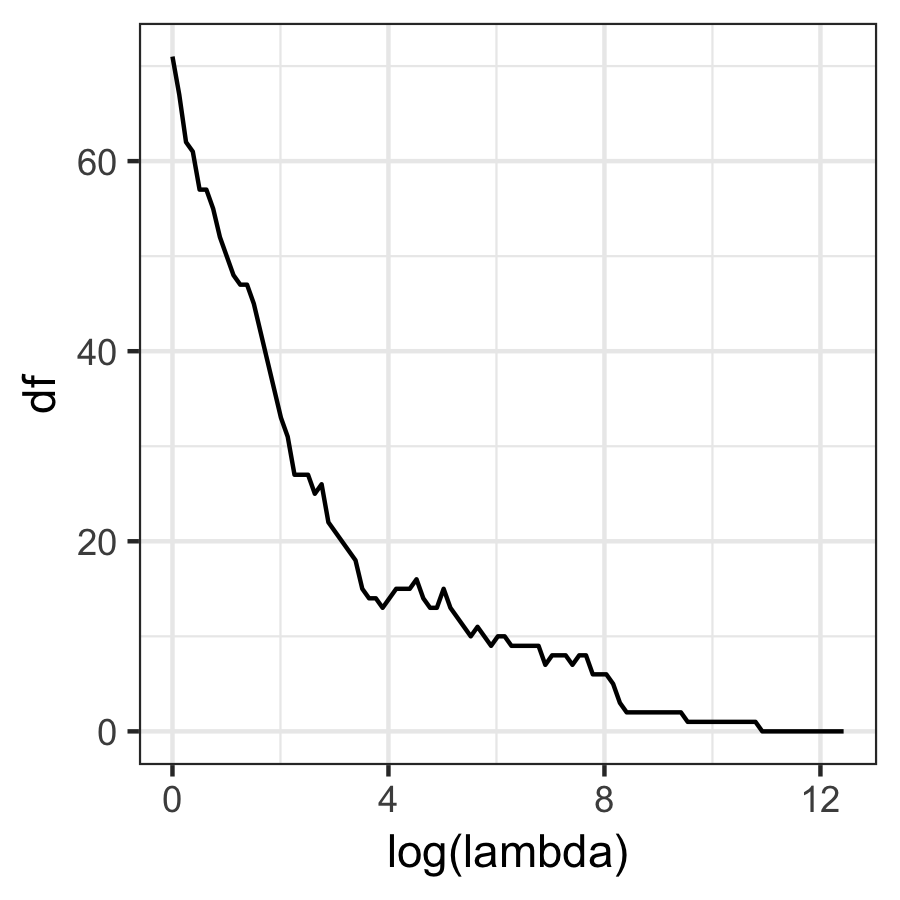
\includegraphics[width = 0.25\linewidth]{Figures/df_by_lambda.png}
		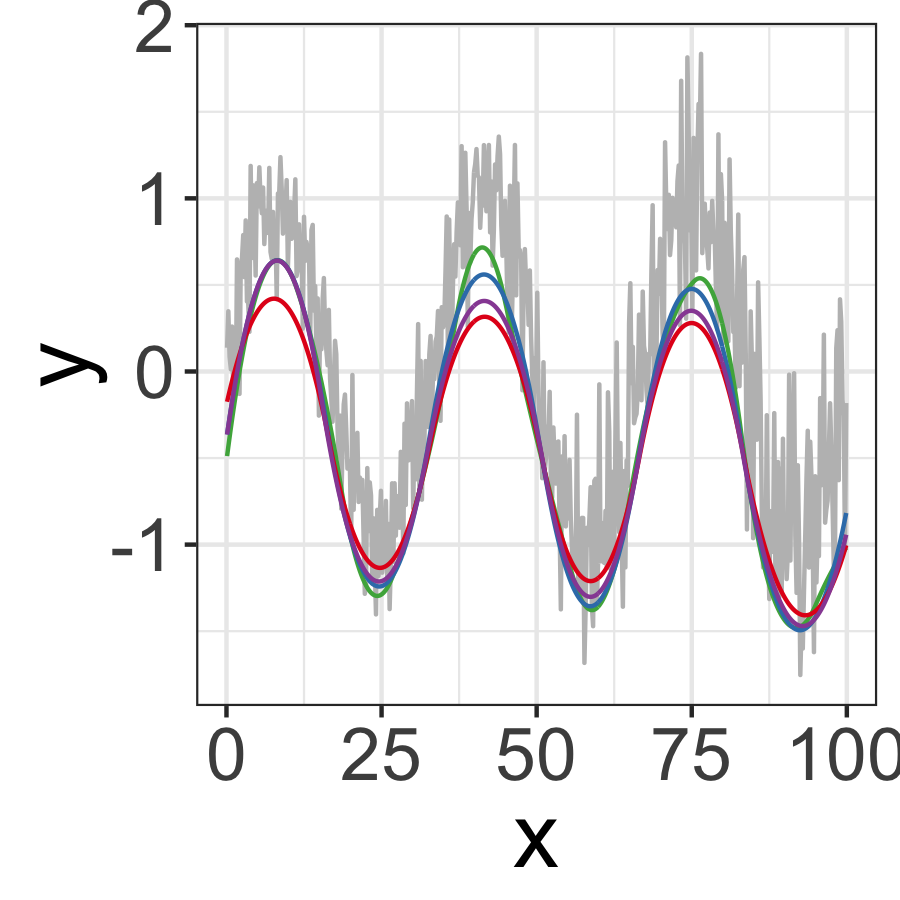
\includegraphics[width = 0.25\linewidth]{Figures/BIC_data.png}
		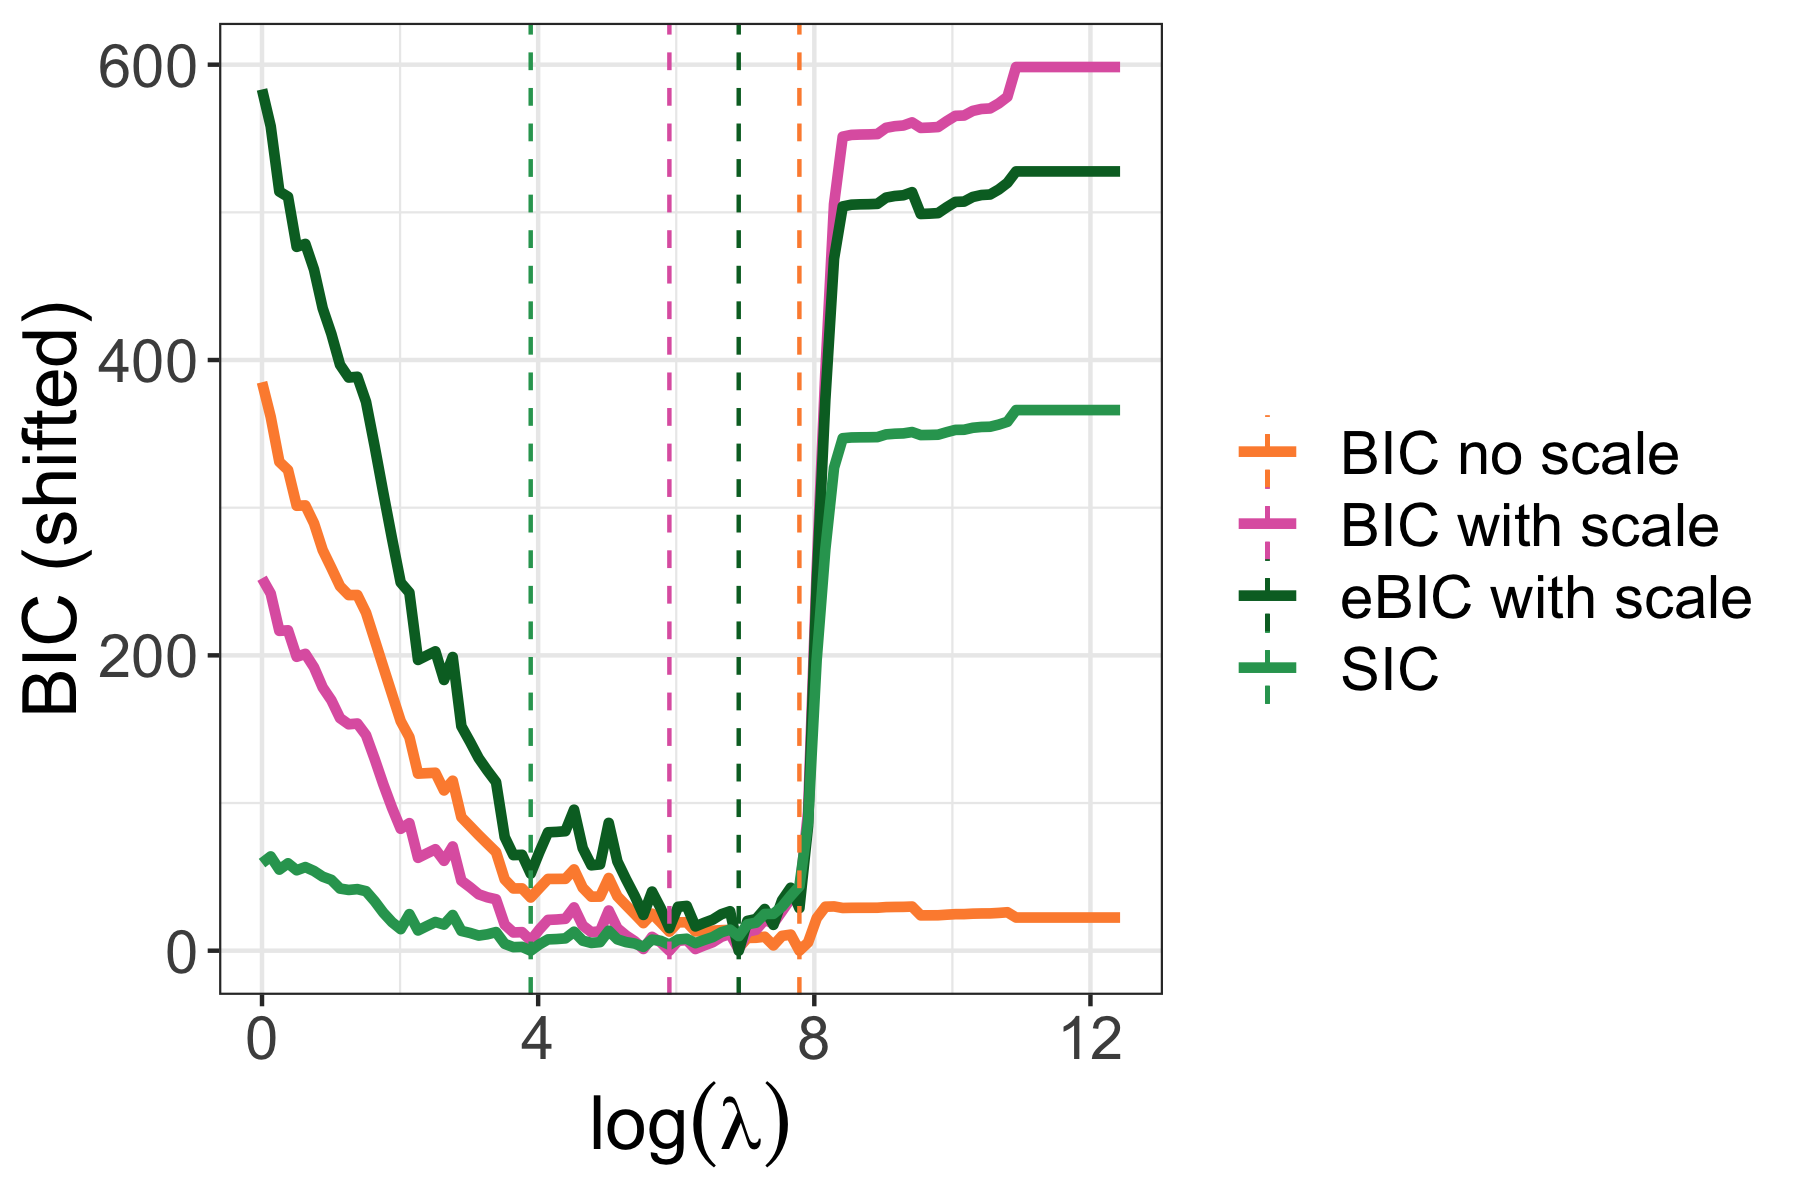
\includegraphics[width = 0.5\linewidth]{Figures/BIC_by_lambda.png} 
		\caption{(Left) Estimated degrees of freedom (number of non-zero elements of $\M{D}\V{\theta}$) as a function of $\log(\lambda)$. (Middle) Estimated 10th quantile trend with regularization parameter chosen using various criteria. (Right) Criteria values as a function of $\log(\lambda)$, vertical lines indicate locations of minima.} 
		\label{fig:BIC}
	\end{figure}

%% ----------------------------------------------------------------------
%% Simulation Studies
%% ----------------------------------------------------------------------
\section{Simulation Studies}
\label{sec:simluation}

	We conduct two simulation studies to compare the performance of our quantile trend filtering method and regularization parameter selection criteria with previously published methods. The first study compares the method's ability to estimate quantiles when the only components of the observed series are a smooth trend and a random component. The second study is based on our application and compares the method's ability to estimate baseline trends and enable peak detection when the time series contains a non-negative signal component in addition to the trend and random component. 
	
	We compare three criteria for choosing the smoothing parameter with our quantile trend filtering method with a single window: \texttt{detrendr\_SIC} $\lambda$ chosen using SIC \Eqn{SIC} \citep{KoenkerNgPortnoy1994}; \texttt{detrendr\_valid}: $\lambda$ is chosen by leaving out every 5th observation as a validation data set and minimizing the check loss function evaluated at the validation data; \texttt{detrendr\_eBIC}:  the proposed scaled eBIC criteria \Eqn{eBIC}.
	
	We also compare the performance of our quantile trend filtering method with three previously published methods: \texttt{npqw} which is the quantile-ll method described in \cite{Racine2017}, code was obtained from the author; \texttt{qsreg} in the \texttt{fields} R package and described in \cite{Oh2011, nychka1995nonparametric}; \texttt{rqss} available in the \texttt{quantreg} package and described in \cite{KoenkerNgPortnoy1994}.  The regularization parameter $\lambda$ for the \texttt{rqss} method is chosen using a grid search and minimizing the SIC criteria as described in \cite{KoenkerNgPortnoy1994}, the regularization parameter for \texttt{qsreg} was chosen using generalized cross-validation based on the quantile criterion \cite{Oh2011}. 
	
%% ----------------------------------------------------------------------
%% Estimating Quantiles
%% ----------------------------------------------------------------------	 
\subsection{Estimating Quantiles}
	\begin{figure}
		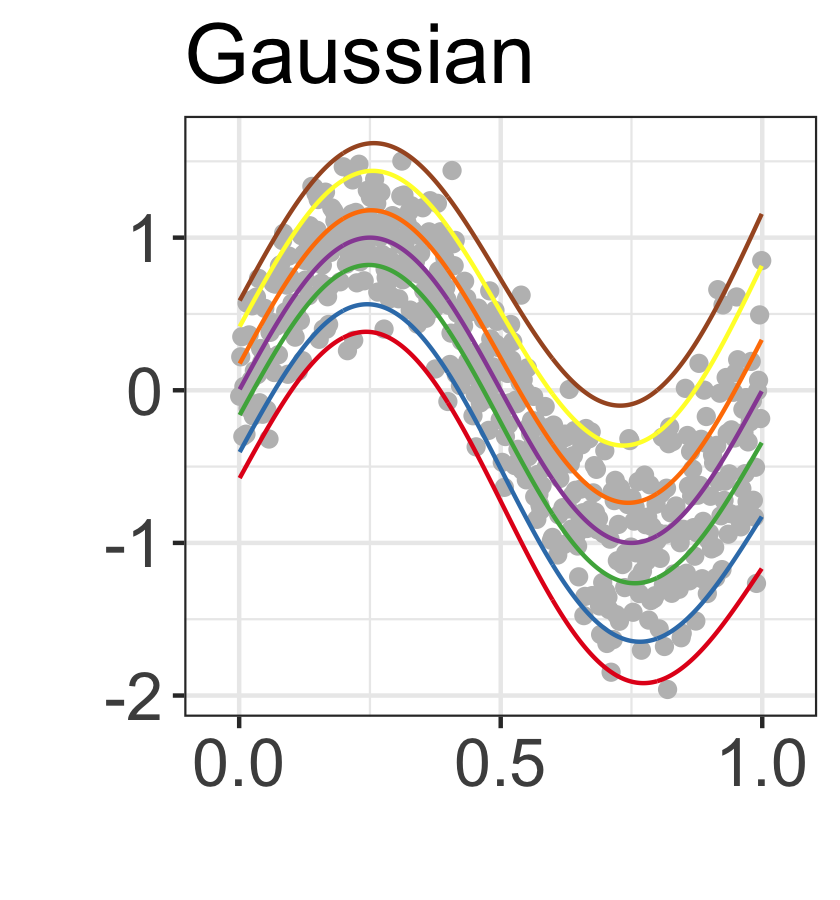
\includegraphics[width=.28\linewidth]{Figures/gaus.png}
		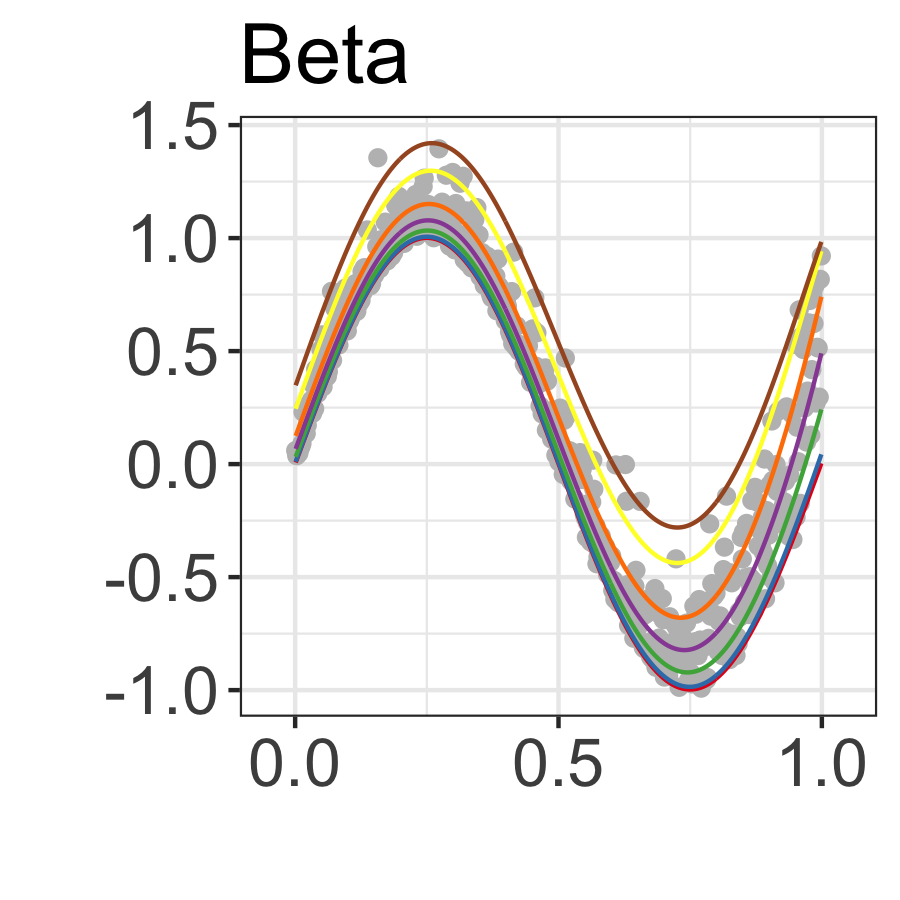
\includegraphics[width=.3\linewidth]{Figures/shapebeta.png}
		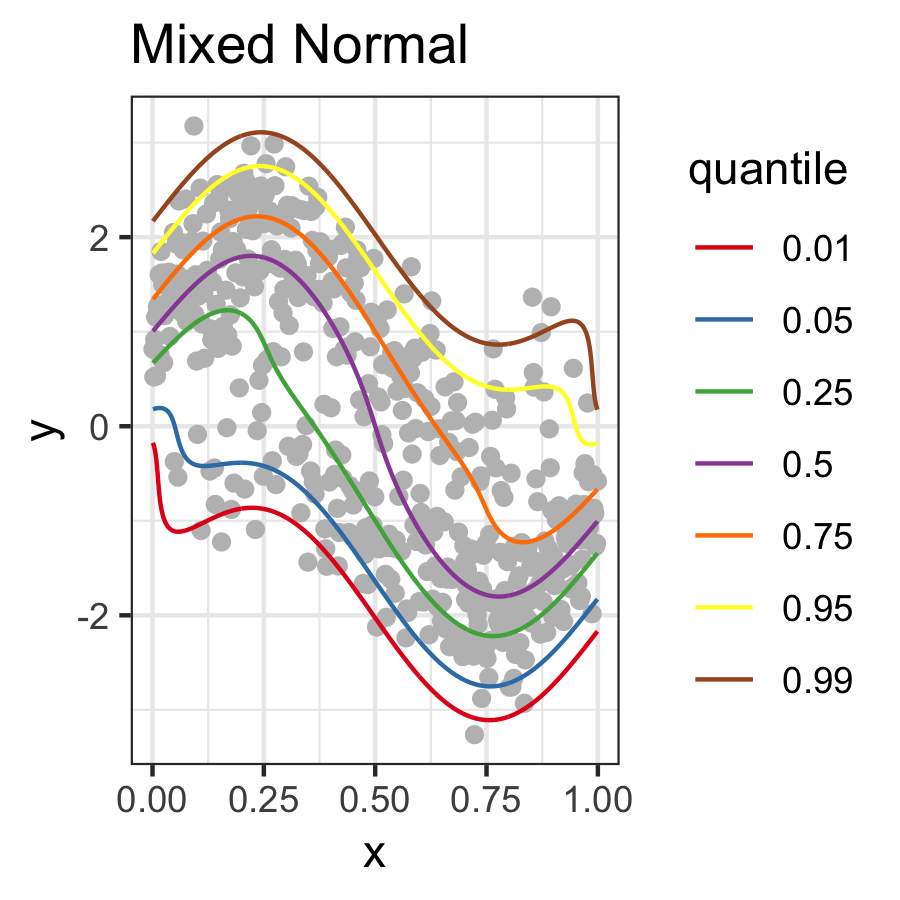
\includegraphics[width=.45\linewidth]{Figures/mixednorm.png}
		\caption{Simulated data with true quantile trends.}			
	\end{figure}

	To compare performance in estimating quantile trends, three simulation designs from \cite{Racine2017} were considered. For all designs $t = 1, \ldots, n$,  $x(t) = t/n$, and the response $\V{y}$ was generated as 
\begin{eqnarray*}
y(t) & = & \sin(2\pi x(t)) + \epsilon(x(t))
\end{eqnarray*}
	The three error distributions considered were 
	\begin{itemize}
		\item Gaussian: $\epsilon(x(t)) \sim N\left(0, \left(\frac{1+x(t)^2}{4}\right)^2\right)$
		\item Beta: $\epsilon(x(t)) \sim Beta(1, 11-10x(t))$
		\item Mixed normal: $\epsilon(x(t))$ is simulated from a mixture of $N(-1,1)$ and  $N(1,1)$ with mixing probability $x(t)$.
	\end{itemize}
	
	One hundred datasets were generated of sizes 300, 500 and 1000. For each method quantile trends were estimated for $\tau = \{0.05, 0.25, 0.5, 0.75, 0.95\}$. Only our detrend methods guarantee non-crossing quantiles. For each quantile trend and method the root mean squared error was calculated as $\mbox{RMSE} = \sqrt{\frac{1}{n}\sum_i (\hat{q}_{\tau}(t_i) - q_\tau(t_i))^2}$. \Fig{quantile_mse} shows the mean RMSE $\pm$ twice the standard error for each method, quantile level, and sample size. 	In all three designs the proposed detrend methods are either better than or comparable to existing methods. Overall the \texttt{detrend\_eBIC} performs best, and especially in the mixed normal design our methods have lower RMSEs for the 5\textsuperscript{th} and 95\textsuperscript{th} quantiles. The \texttt{npqw} method performs particularly poorly in the mixed normal design due to the fact that it assumes the data come from a scale-location model, which is violated in this case. 
	
	\begin{figure}
		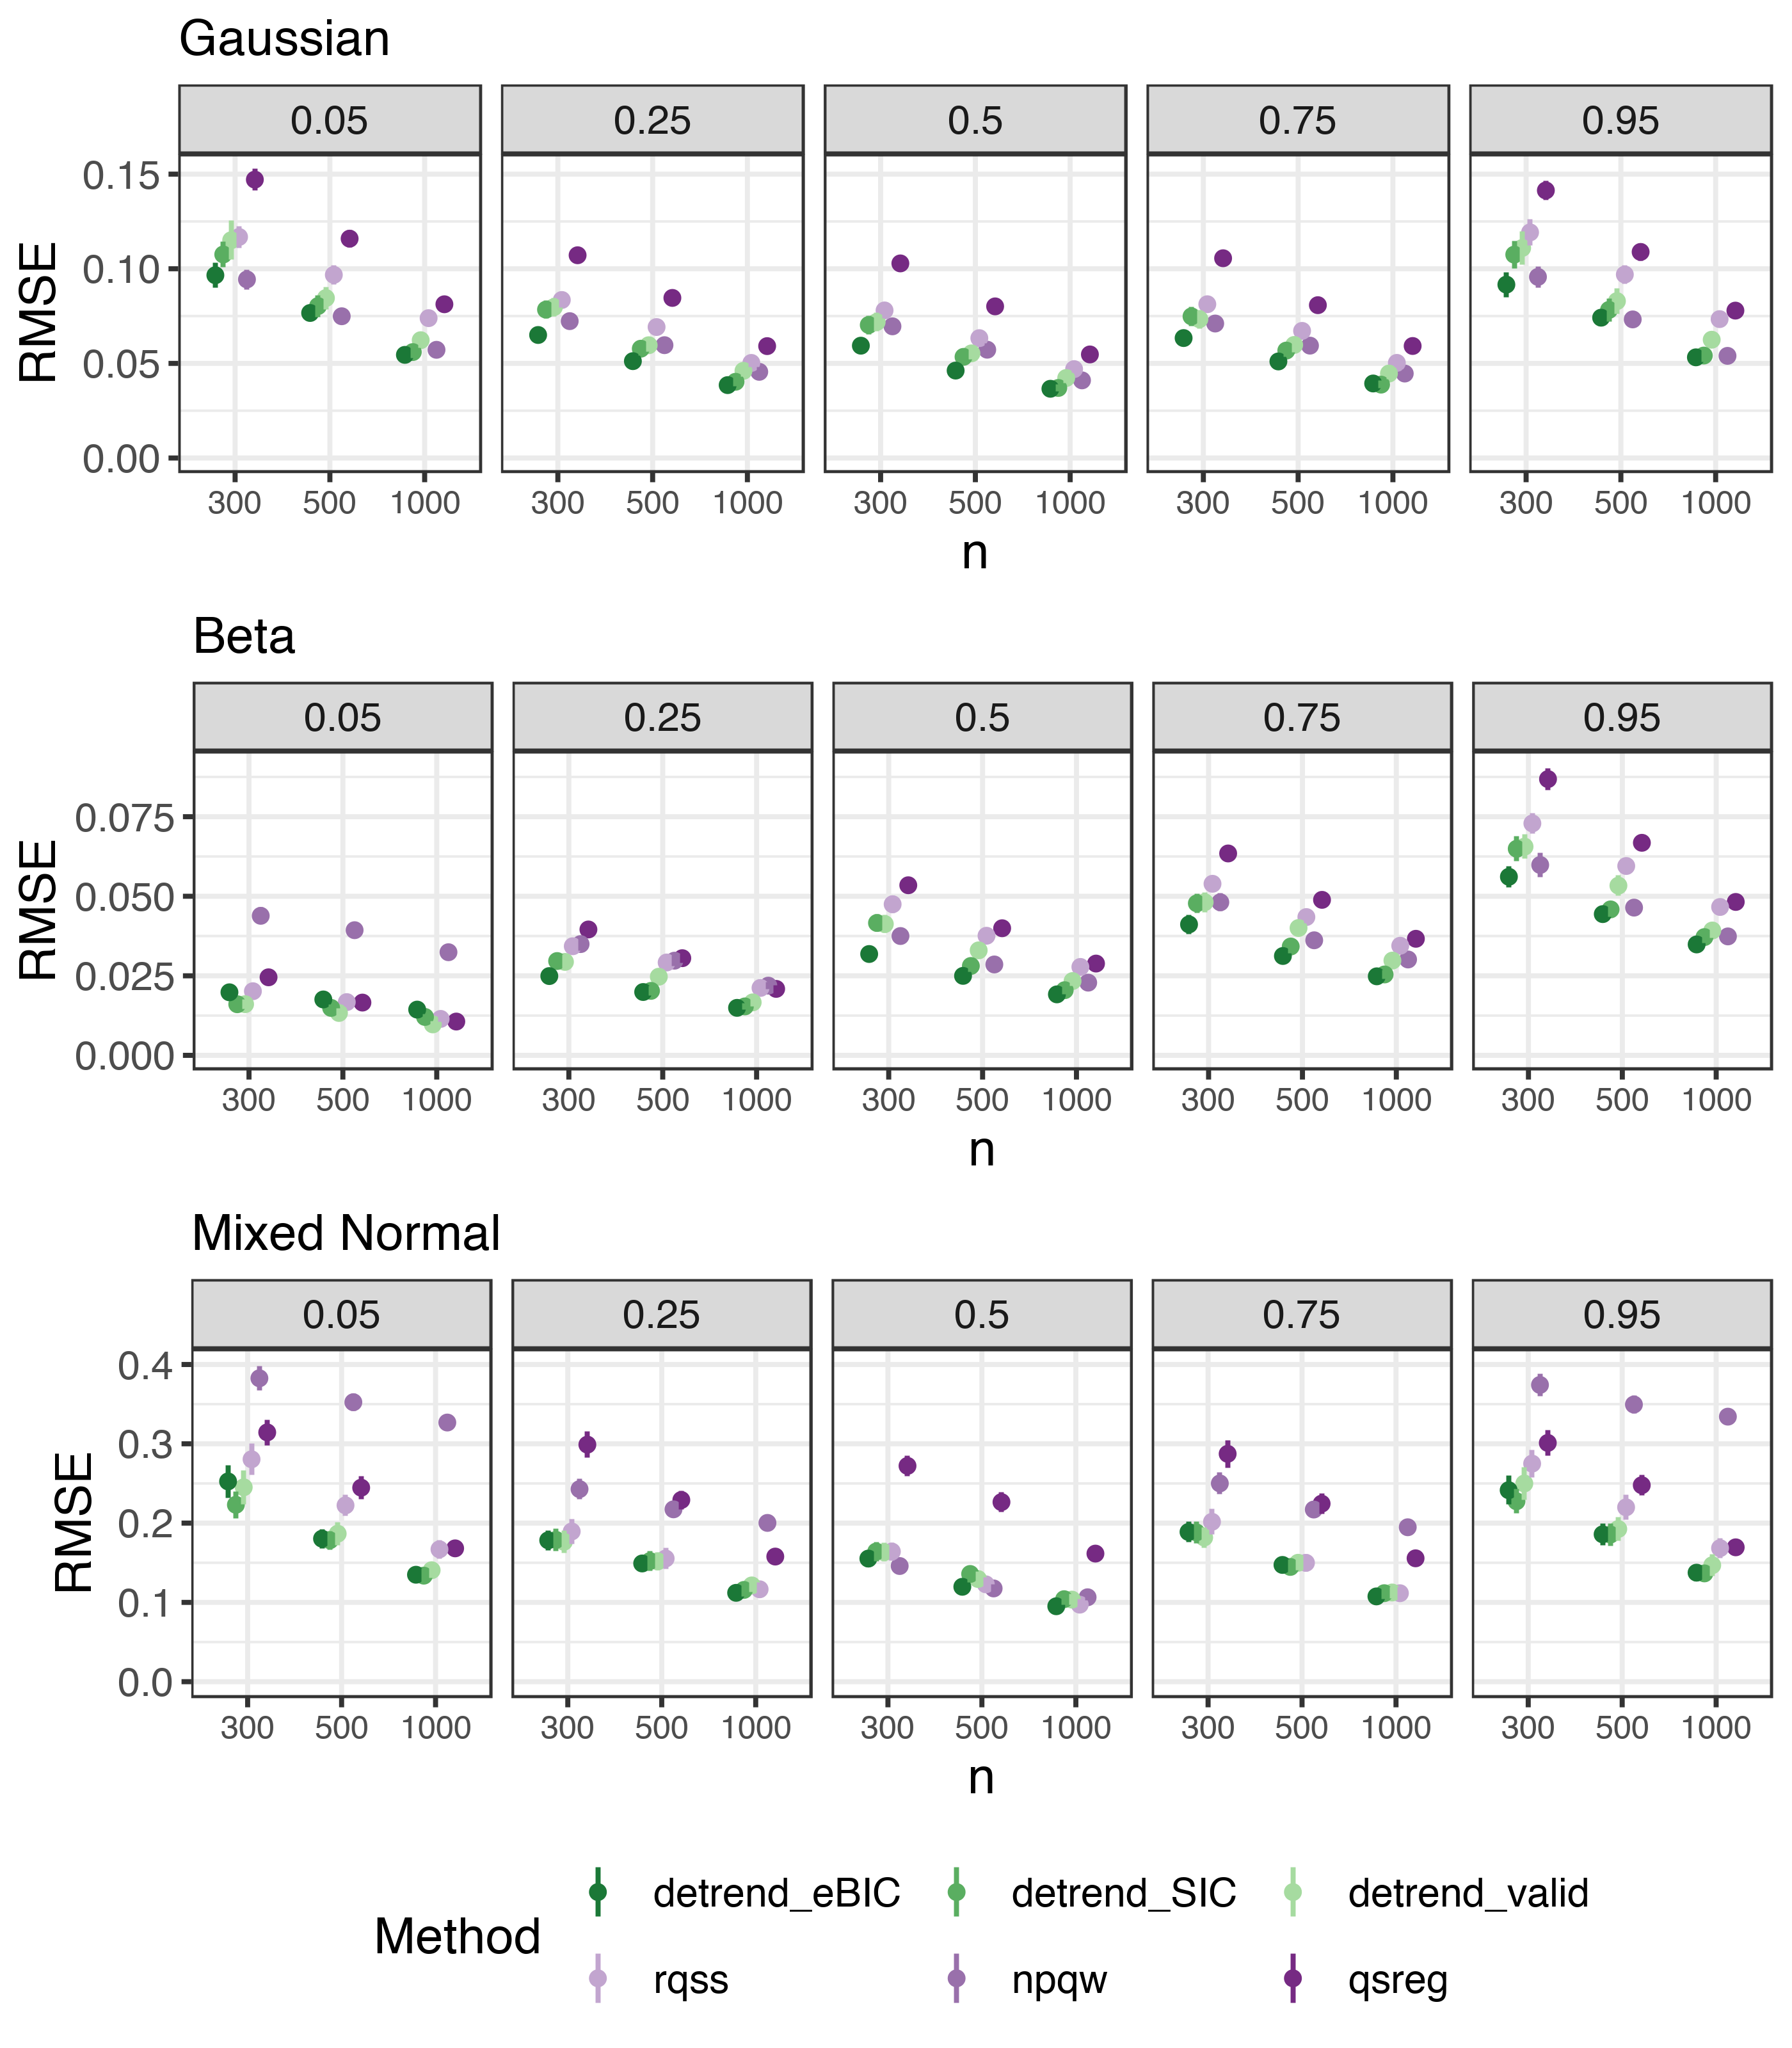
\includegraphics[width=\linewidth]{Figures/sim_metrics.png}	
		\caption{RMSE by design, method, quantile and data size. Points and error bars represent mean RMSE $\pm$ twice the standard error.}
		\label{fig:quantile_mse}
	\end{figure}

%% ----------------------------------------------------------------------
%% Peak Detection
%% ----------------------------------------------------------------------
\subsection{Peak Detection}
%	\begin{figure}[h]
%		\caption{Example of simulated peaks, baseline, and observed measurements.}
%		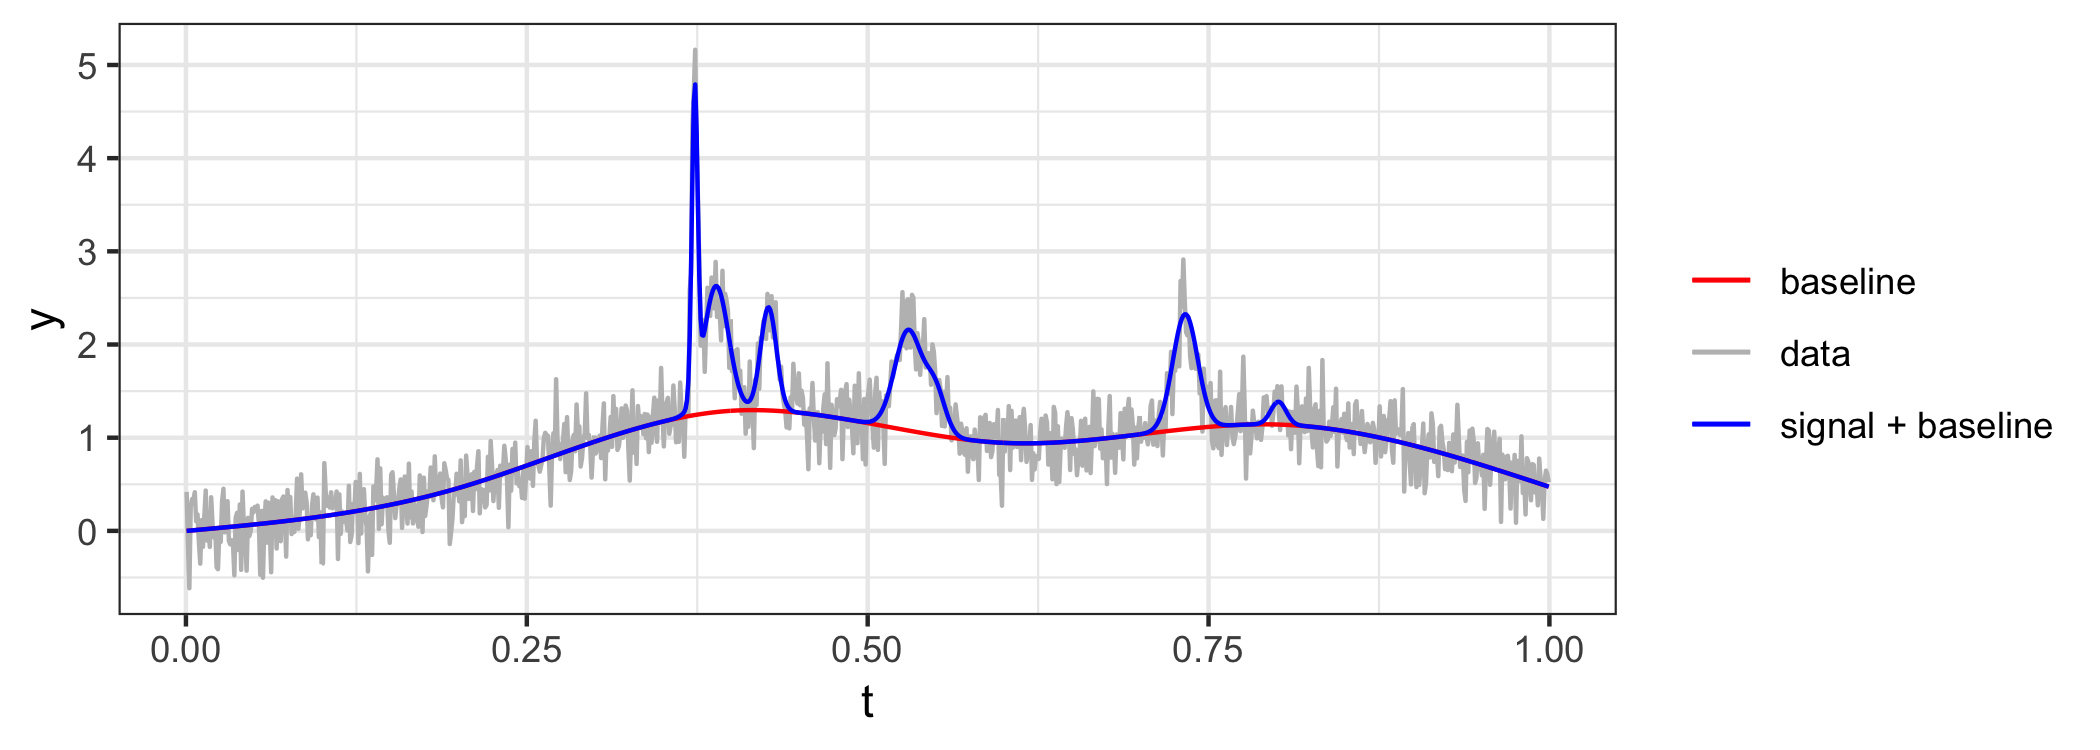
\includegraphics[width = \linewidth]{Figures/ex_peaks.png}
%	\end{figure}
	We use another simulation design based on our motivating application. We assume that the measured data can be represented by 
	\begin{eqnarray*}
	y(t_i) & = & \theta(t_i) + s(t_i) + \VE{\varepsilon}{i},
	\end{eqnarray*}  
	where $t_i = i$ for $i = 1, ..., n$, $\theta(t)$ is the drift component that varies smoothly over time, $s(t)$ is the true signal at time $t$, and $\VE{\varepsilon}{i}$ are i.i.d.\@ errors distributed as $N(0, 0.25^2)$. We generate $\theta(t)$ using cubic natural spline basis functions with degrees of freedom sampled from a Poisson distribution with mean parameter equal to $n/100$,  and coefficients drawn from an exponential distribution with rate 1. The true signal function $s(t)$ is assumed to be zero with peaks generated using the Gaussian density function. The number of peaks is sampled from a binomial distribution with size equal to $n$ and probability equal to $0.005$ with location parameters uniformly distributed between $1$ and $n-1$ and bandwidths uniformly distributed between $2$ and $12$. The simulated peaks were multiplied by a factor that was randomly drawn from a normal distribution with mean 20 and standard deviation of 4. One hundred datasets were generated for each $n=\{500, 1000, 2000, 4000\}$. We compare the ability of the methods to estimate the true quantiles of $y(t_i)-s(t_i)$  for $\tau \in \{0.01, 0.05, 0.1\}$ and calculate the RMSE (\Fig{peaks_rmse}). In this simulation study, our proposed method \texttt{detrend\_eBIC} method substantially outperforms the others. The \texttt{qsreg} method is comparable to the \texttt{detrend\_eBIC} method on the smaller datasets, but its performance deteriorates as the data size grows. The \texttt{npqw} and \texttt{detrend\_valid} methods both perform poorly on this design. 
	
	\begin{figure}
		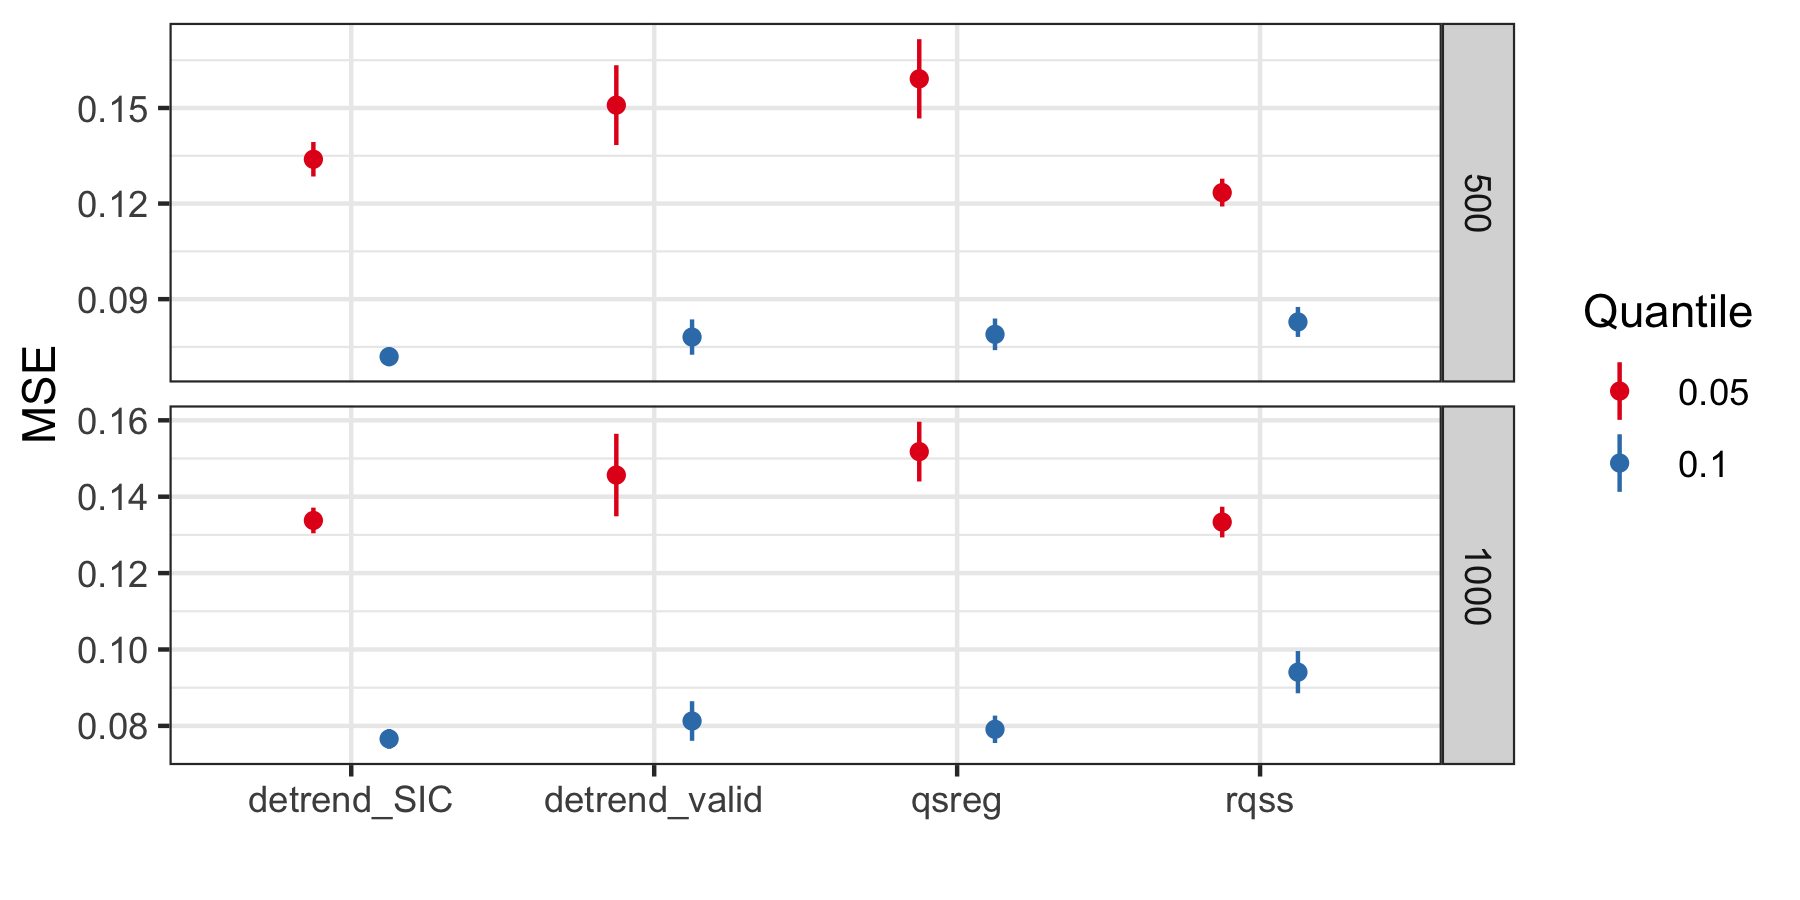
\includegraphics[width = \linewidth]{Figures/peaks_mse.png}	
		\caption{RMSE by method, quantile, and data size for peaks design.}
		\label{fig:peaks_rmse}
	\end{figure}
	
	While minimizing RMSE is desirable in general, in our application, the primary metric of success is accurately classifying observations $\VE{y}{i}$ as signal or no signal. To evaluate the accuracy of our method compared to other methods we define true signal as any time point when the simulated peak value is greater than 0.5. We compare three different quantiles for the baseline estimation and four different thresholds for classifying the signal after subtracting the estimated baseline from the observations.  \Fig{peaks_class_eg} shows an illustration of the observations classified as signal after subtracting the baseline trend compared to the ``true signal." Let $\delta_i \in \{0,1\}$ be the vector of true signal classifications and $\hat{\delta}_i \in \{0,1\}$ be the vector of estimated signal classifications, namely $\hat{\delta}_i = \One(\VE{y}{i} - \hat{\theta}_{i} > 0.5)$.
	
	
	To compare the resulting signal classifications, we calculate the class averaged accuracy (CAA), which is defined as
	\begin{eqnarray*}
	\mbox{CAA} & = & \frac{1}{2}\left[\frac{\sum_{i=1}^n \One[\delta_i = 1 \cap \hat{\delta}_i = 1]}{\sum_{i=1}^n \One[\delta_i = 1]} + \frac{\sum_{i=1}^n \One[\delta_i = 0 \cap \hat{\delta}_i=0]}{\sum_{t=i=1}^n \One[\delta_i = 0]}\right].
	\end{eqnarray*}  
	We use this metric because our classes tend to be very imbalanced with many more zeros than ones. The CAA metric will give a score of 0.5 for random guessing and also for trivial classifiers such as $\hat{\delta}_i = 0$ for all $i$. 

	Our \texttt{detrend\_BIC} method performs the best overall in terms of both RMSE and CAA. While \texttt{qsreg} was competitive with our method in some cases, in the majority of cases the largest CAA values for each threshold were produced using the \texttt{detrend\_eBIC} method with the 1\textsuperscript{st} or 5\textsuperscript{th} quantiles. 
	
	\begin{figure}[h!]
		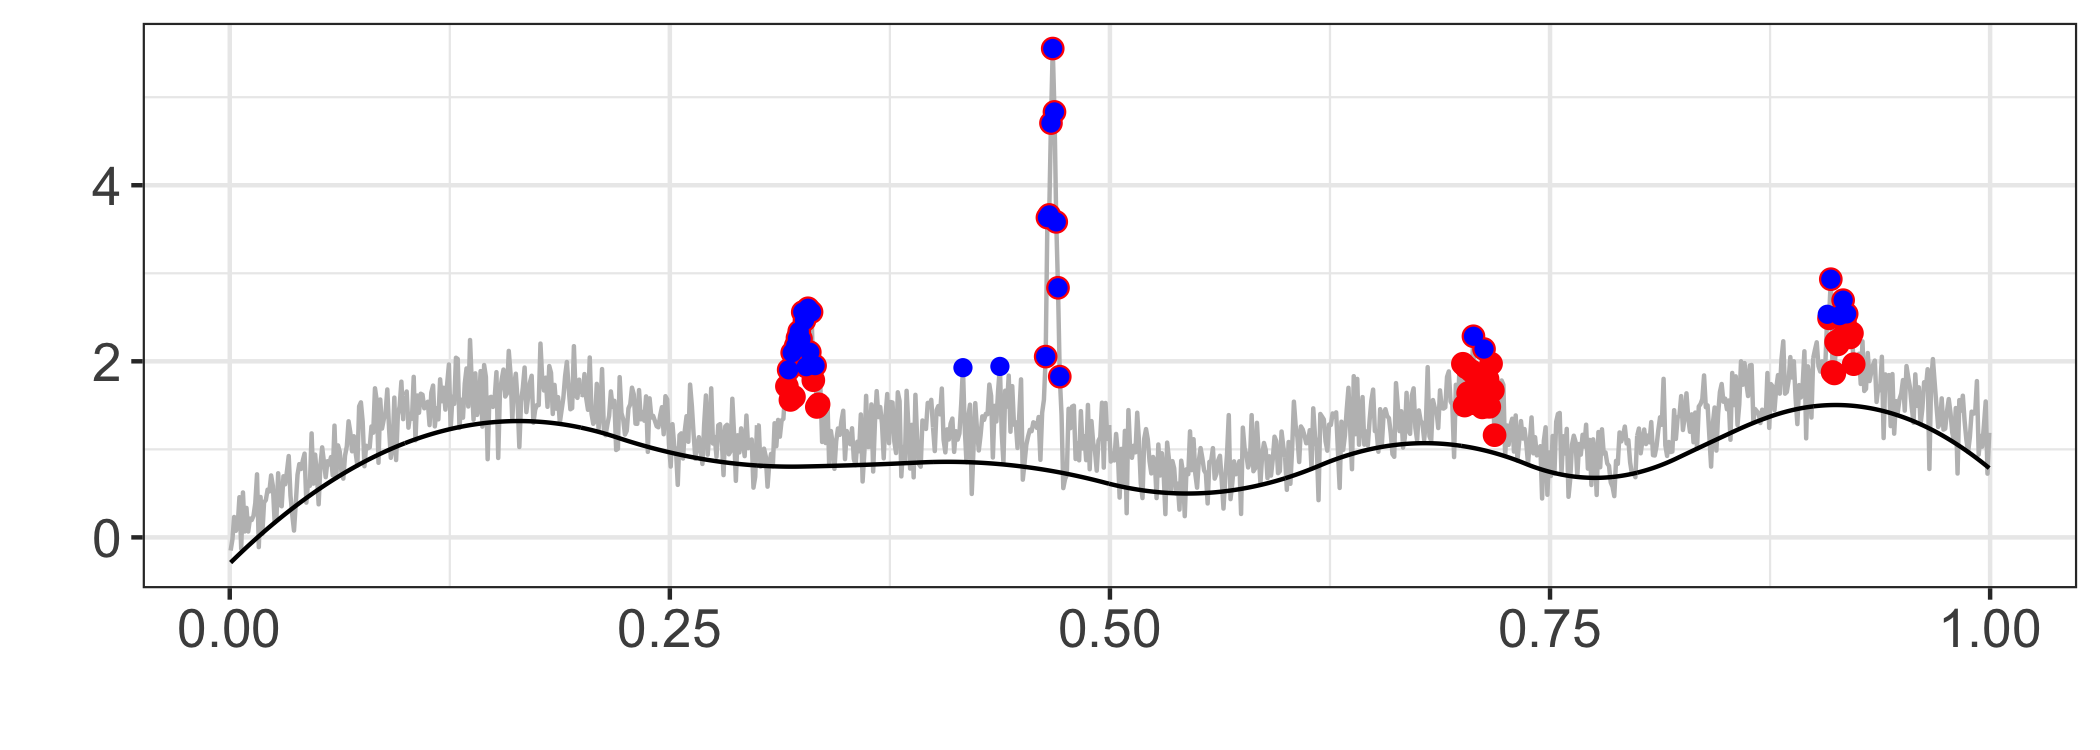
\includegraphics[width = \linewidth]{Figures/peaks_eg_class.png}
		\caption{Example signal classification using threshold. Red indicates true signal $>0.5$, blue indicates observations classified as signal after baseline removal using \texttt{detrend\_eBIC} and a threshold of 1.2.}
		\label{fig:peaks_class_eg}
	\end{figure}
	

	\begin{figure}[h!]
		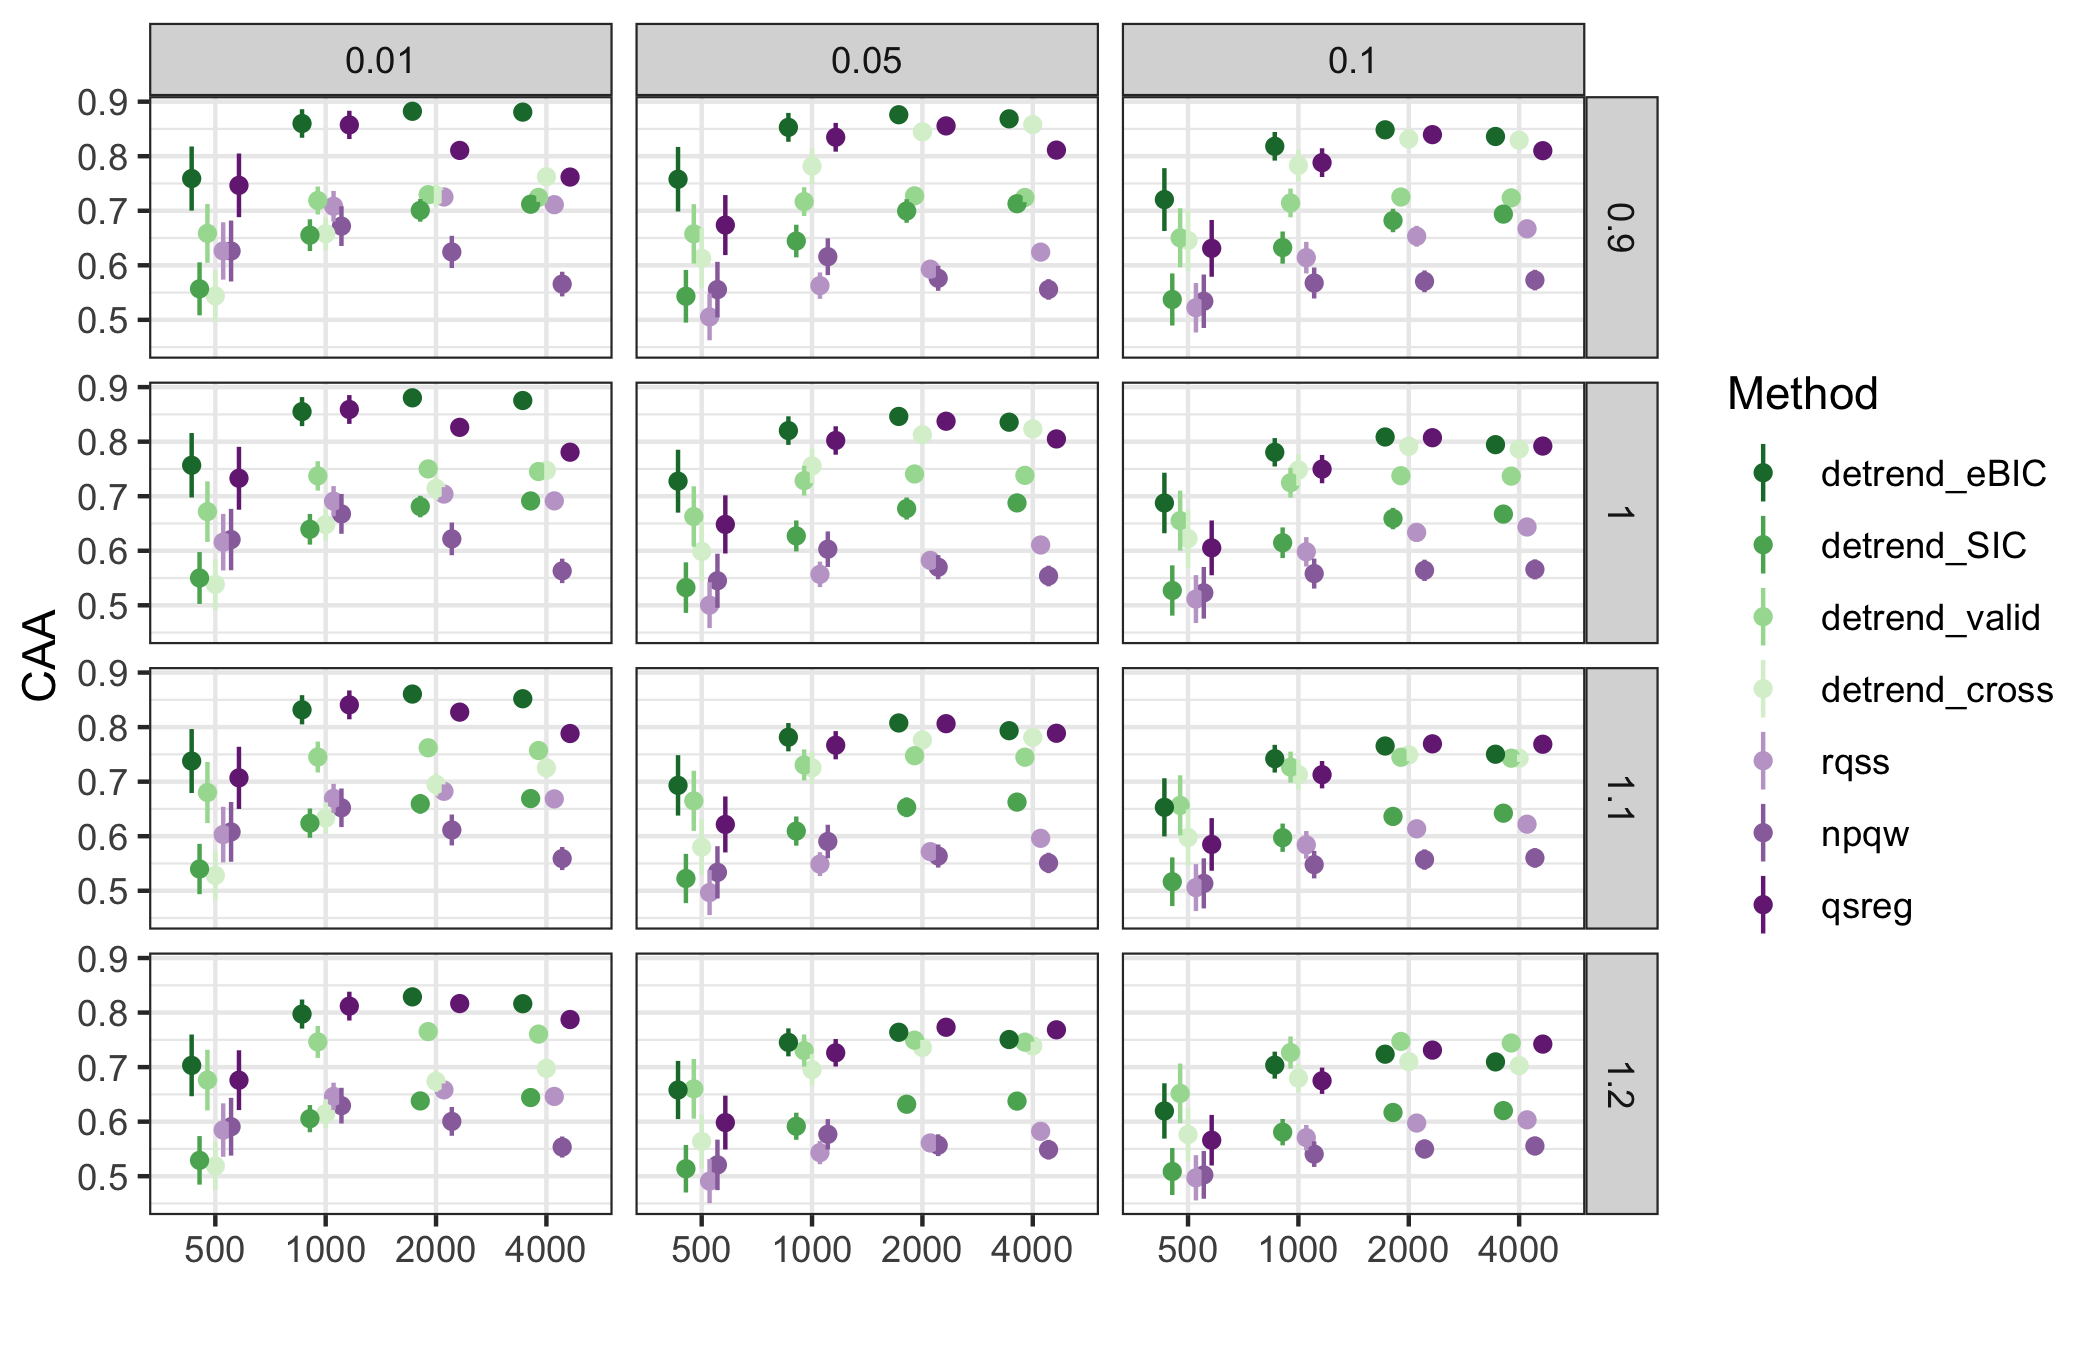
\includegraphics[width = \linewidth]{Figures/peaks_CAA.png}
		\caption{Class averaged accuracy by threshold, data size, and method (1 is best 0.5 is worst).}
	\end{figure}


	\FloatBarrier

%% ----------------------------------------------------------------------
%% Application
%% ----------------------------------------------------------------------	
\section{Application in Air Quality Monitoring}

	\label{sec:application}
	The low-cost ``SPod" air quality sensors output a time series that includes a slowly varying baseline, 
	the sensor response to pollutants, and high frequency random noise. These sensors are used to monitor pollutant concentrations at the fence lines of industrial facilities and detect time points when high concentrations are present. Ideally, three co-located and time aligned sensors (as shown in \Fig{raw_spod}) responding to a pollutant plume would result in the same signal classification after baseline trend removal and proper threshold choice. 

	
	\begin{figure}
		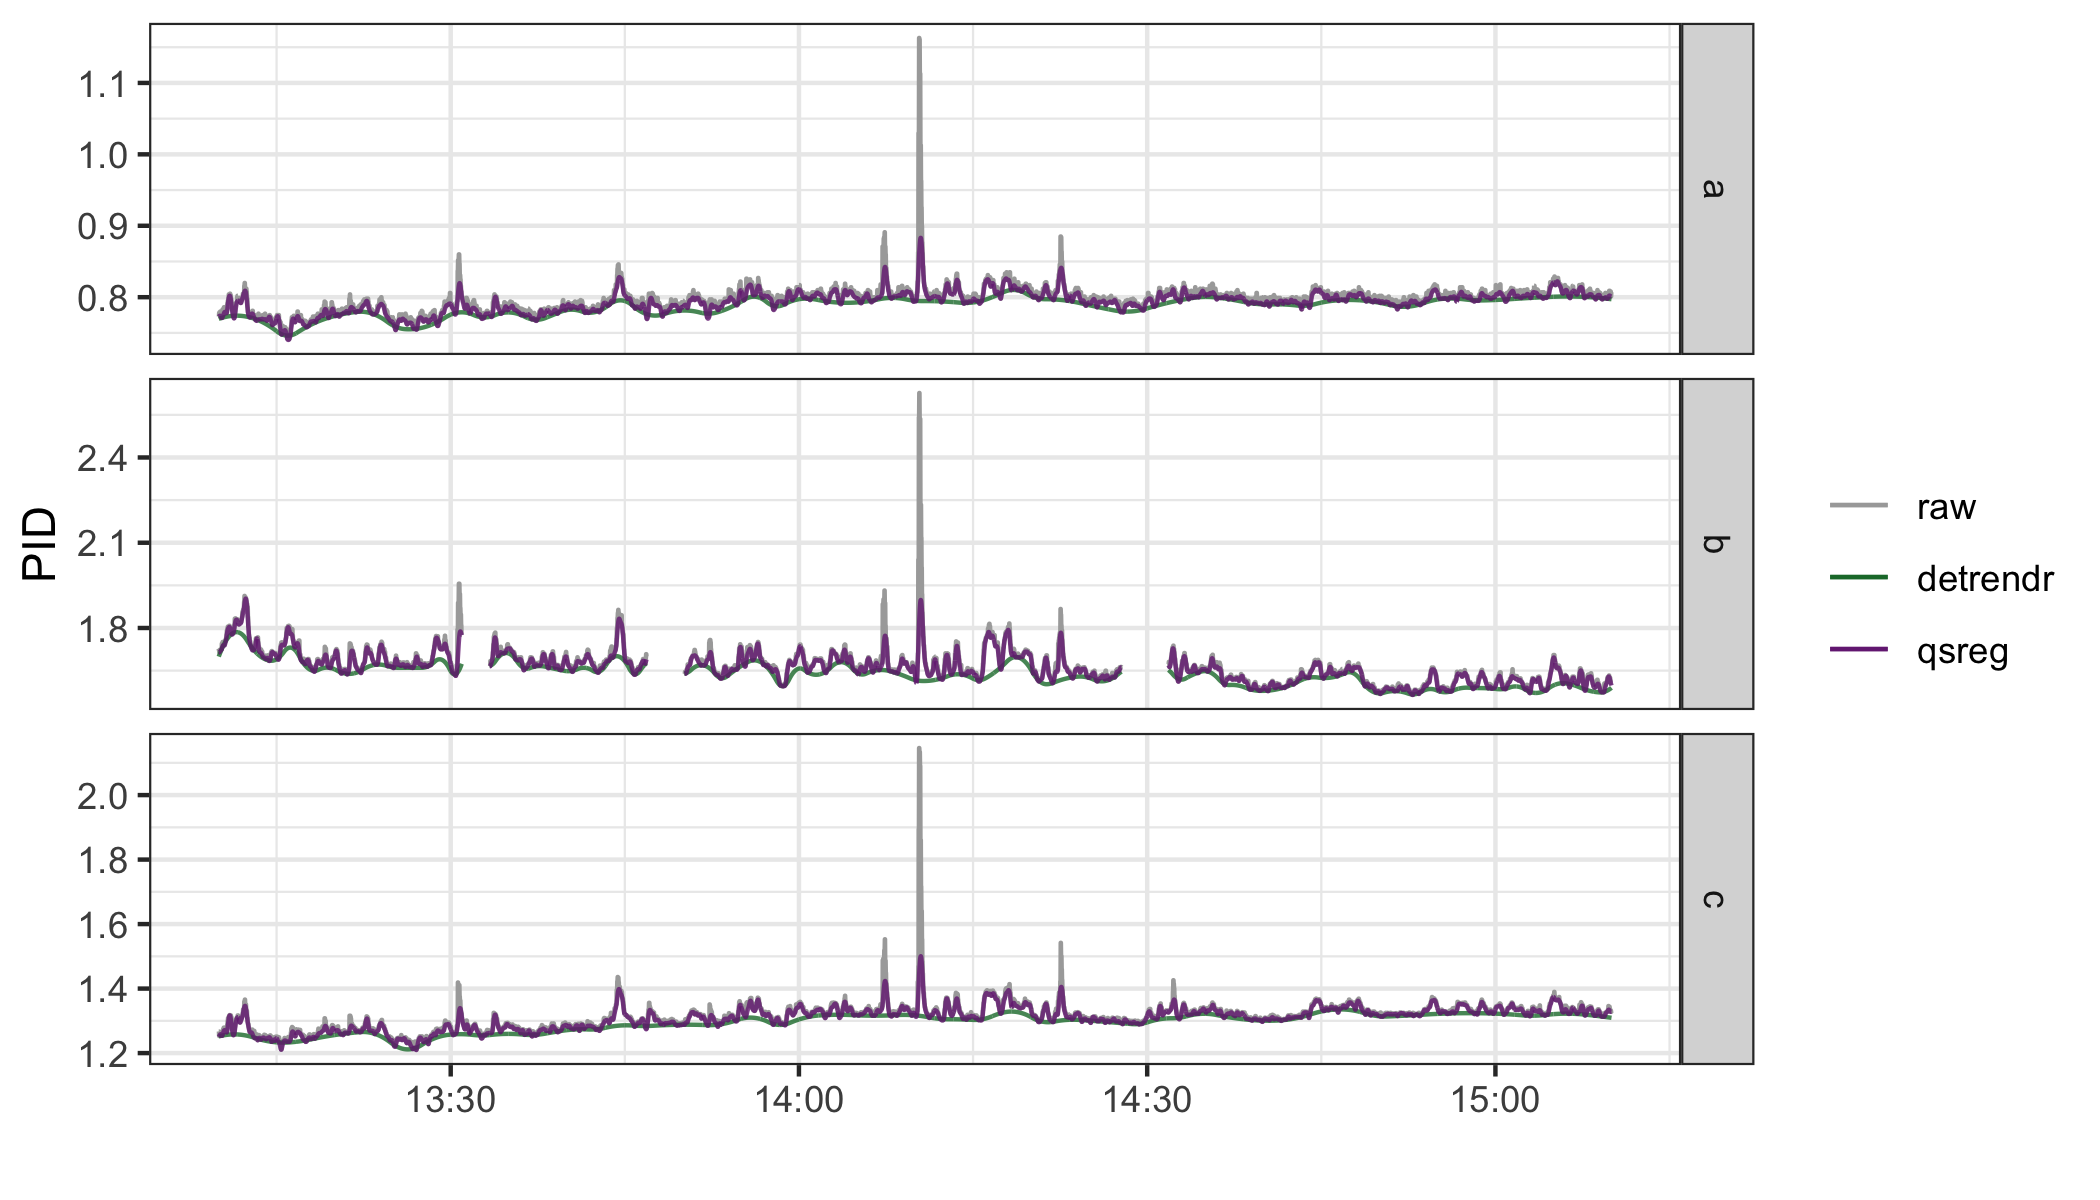
\includegraphics[width = \linewidth]{Figures/short_trends.png}
		\caption{Estimated 15\textsuperscript{th} quantile trends on subset of the data using \texttt{qsreg} and \texttt{detrend\_eBIC}.} 
		\label{fig:short-trends}
	\end{figure}

	We compare our \texttt{detrend\_eBIC} method with the \texttt{qsreg} method on a subset of the SPod data (n=6000) since the \texttt{qsreg} method cannot handle all 24 hours simultaneously. We estimate the baseline trend using the 10\textsuperscript{th} and 15\textsuperscript{th} quantiles and compare three thresholds for classifying signal. The thresholds are calculated using the median plus a multiple of the median absolute deviation \Eqn{MAD} of the detrended series. 
	\begin{eqnarray}
	\label{eq:MAD}
	\mbox{MAD} = \mbox{median}\lVert y-\tilde{y}\rVert,
	\end{eqnarray}
	where $\tilde{y}$ is the median of $y$. Given a method, quantile level, and MAD multiple, we estimate the quantile trend for each of the sensors and subtract it from the observations. We then calculate the threshold using the median plus the MAD multiple of the corrected series and classify the corrected series based on the threshold. \Fig{short-trends} shows an example of the estimated baseline fit for each method, while \Fig{rugplot} shows the series after subtracting the \texttt{detrend\_eBIC} estimate of the 15\textsuperscript{th} quantile and classifying the signal using a MAD multiple of 3. 
	 
 	\begin{figure}
	 	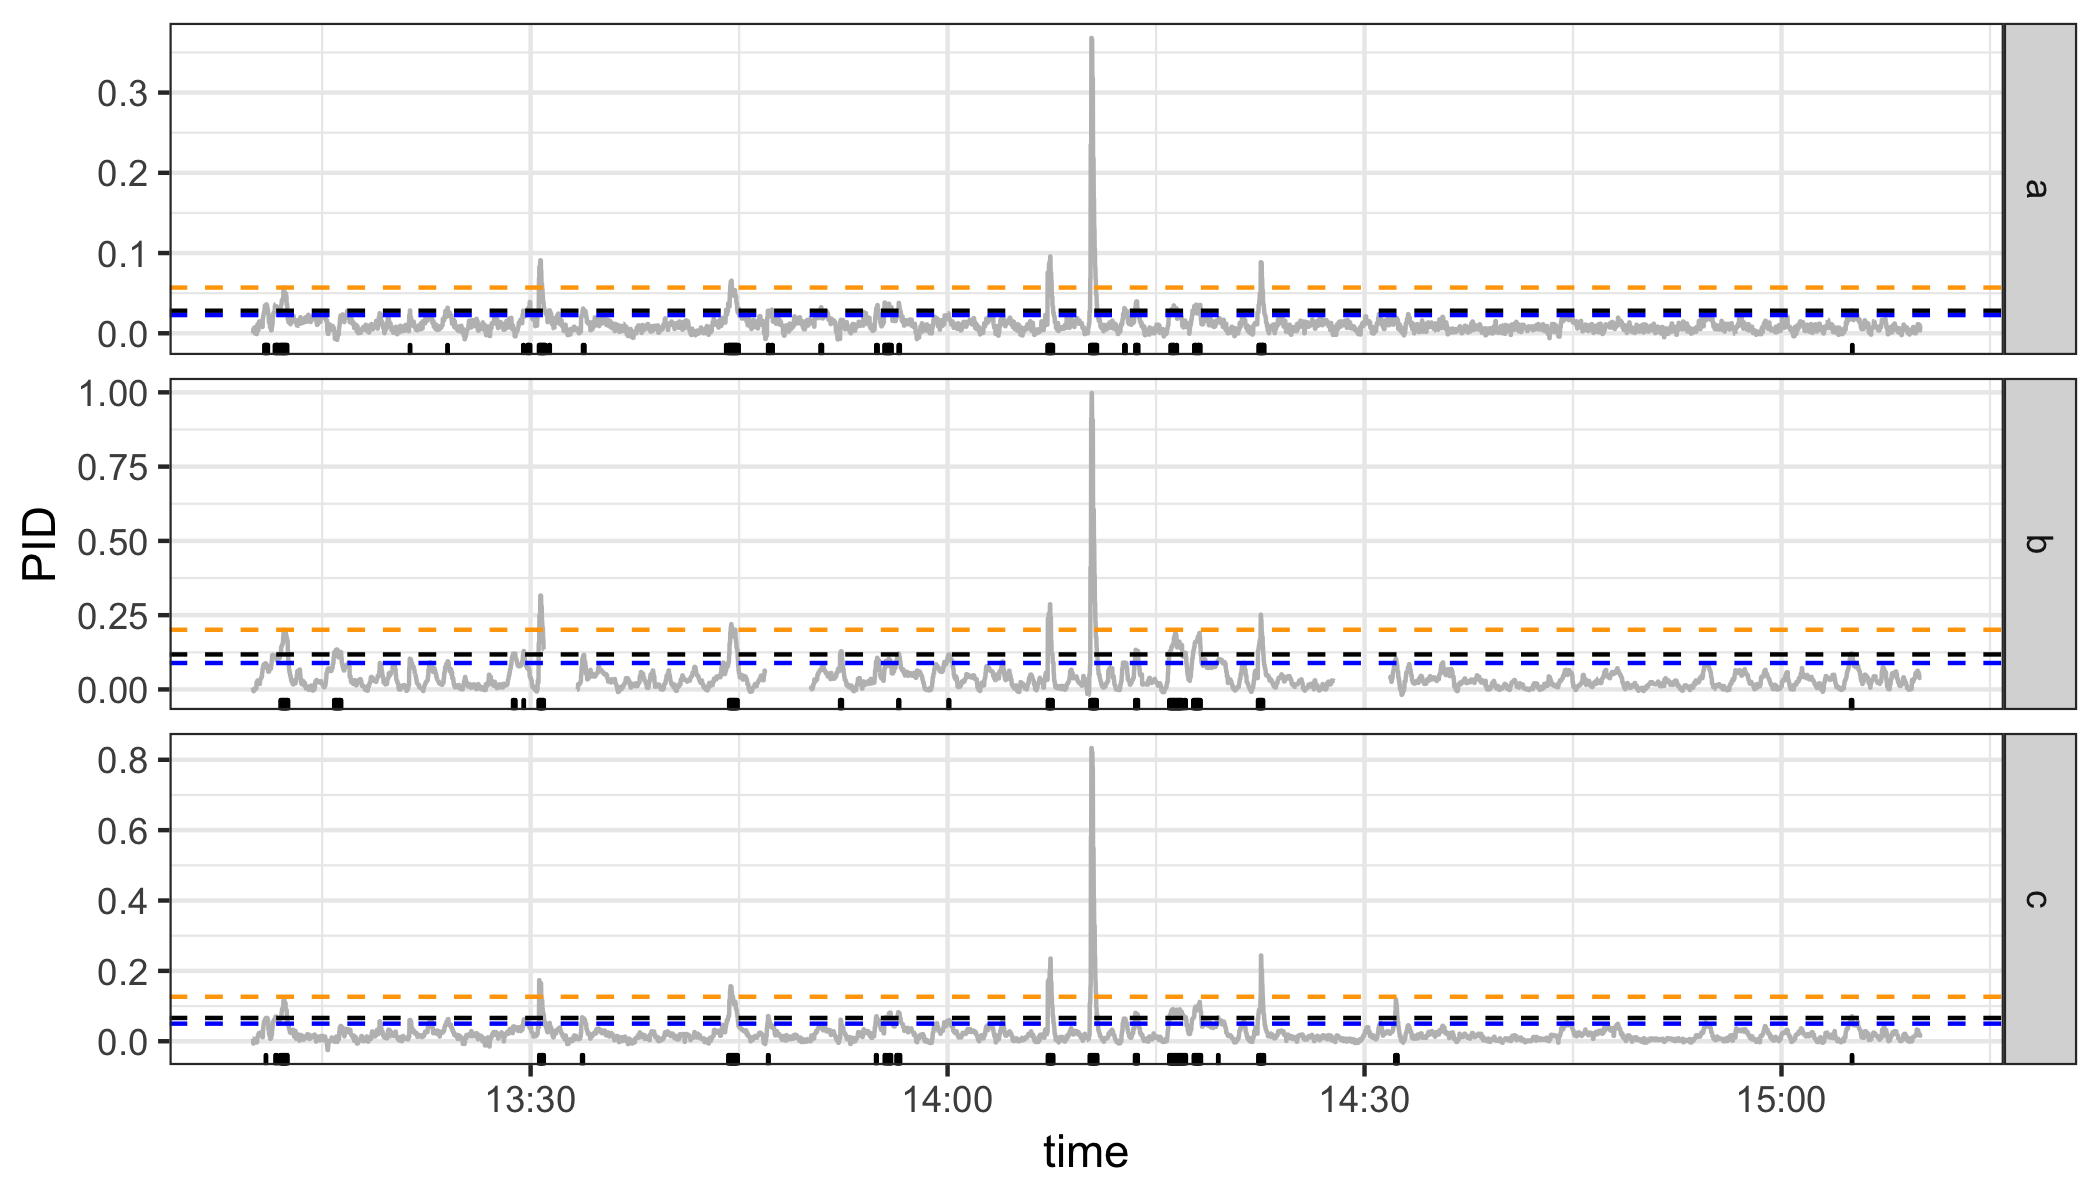
\includegraphics[width = \linewidth]{Figures/corrected_rugplot.png}
	 	\caption{Rugplot showing locations of signal after baseline removal using detrendr estimate of 15th quantile. Horizontal dashed lines represent the thresholds.}
	 	\label{fig:rugplot}
	 \end{figure}
	 
	Given the signal classifications for SPods a and b, $\delta^{(a)}_i \in \{0,1\}$ and $\delta^{(b)}_i\in\{0,1\}$, we want to compare the similarity between the two classifications. One metric for evaluating the distance between two classifications is the variation of information (VI): 
	\begin{eqnarray*}
	r_{ij} & = & \frac{1}{n}\sum_t \One\left(\delta^{(a)}_i = i  \cap \delta^{(b)}_i = j\right)\\
	\VI(s_a, s_b) & = & -\sum_{i,j} r_{ij} \left[ \log \left(\frac{r_{ij}}{\frac{1}{n}\sum_t \One(\delta^{(a)}_i = i)}\right) + 
	\log \left(\frac{r_{ij}}{\frac{1}{n}\sum_t \One(\delta^{(b)}_i = j)}\right) \right]
	\end{eqnarray*}		
	The $\VI$ is a distance metric for measuring similarity of classifications and will be 0 if the classifications are identical and increase as the classifications become more different.  \Fig{vi} shows plots the VIs by method, quantile, and trend. In all cases, our \texttt{detrend} method results in classifications that are more similar than those from the \texttt{qsreg} method. \Fig{short-trends} and \Fig{rugplot} illustrate that our method results in a smoother baseline estimate which improves signal classification. 
		
	\begin{figure}
		\centering
		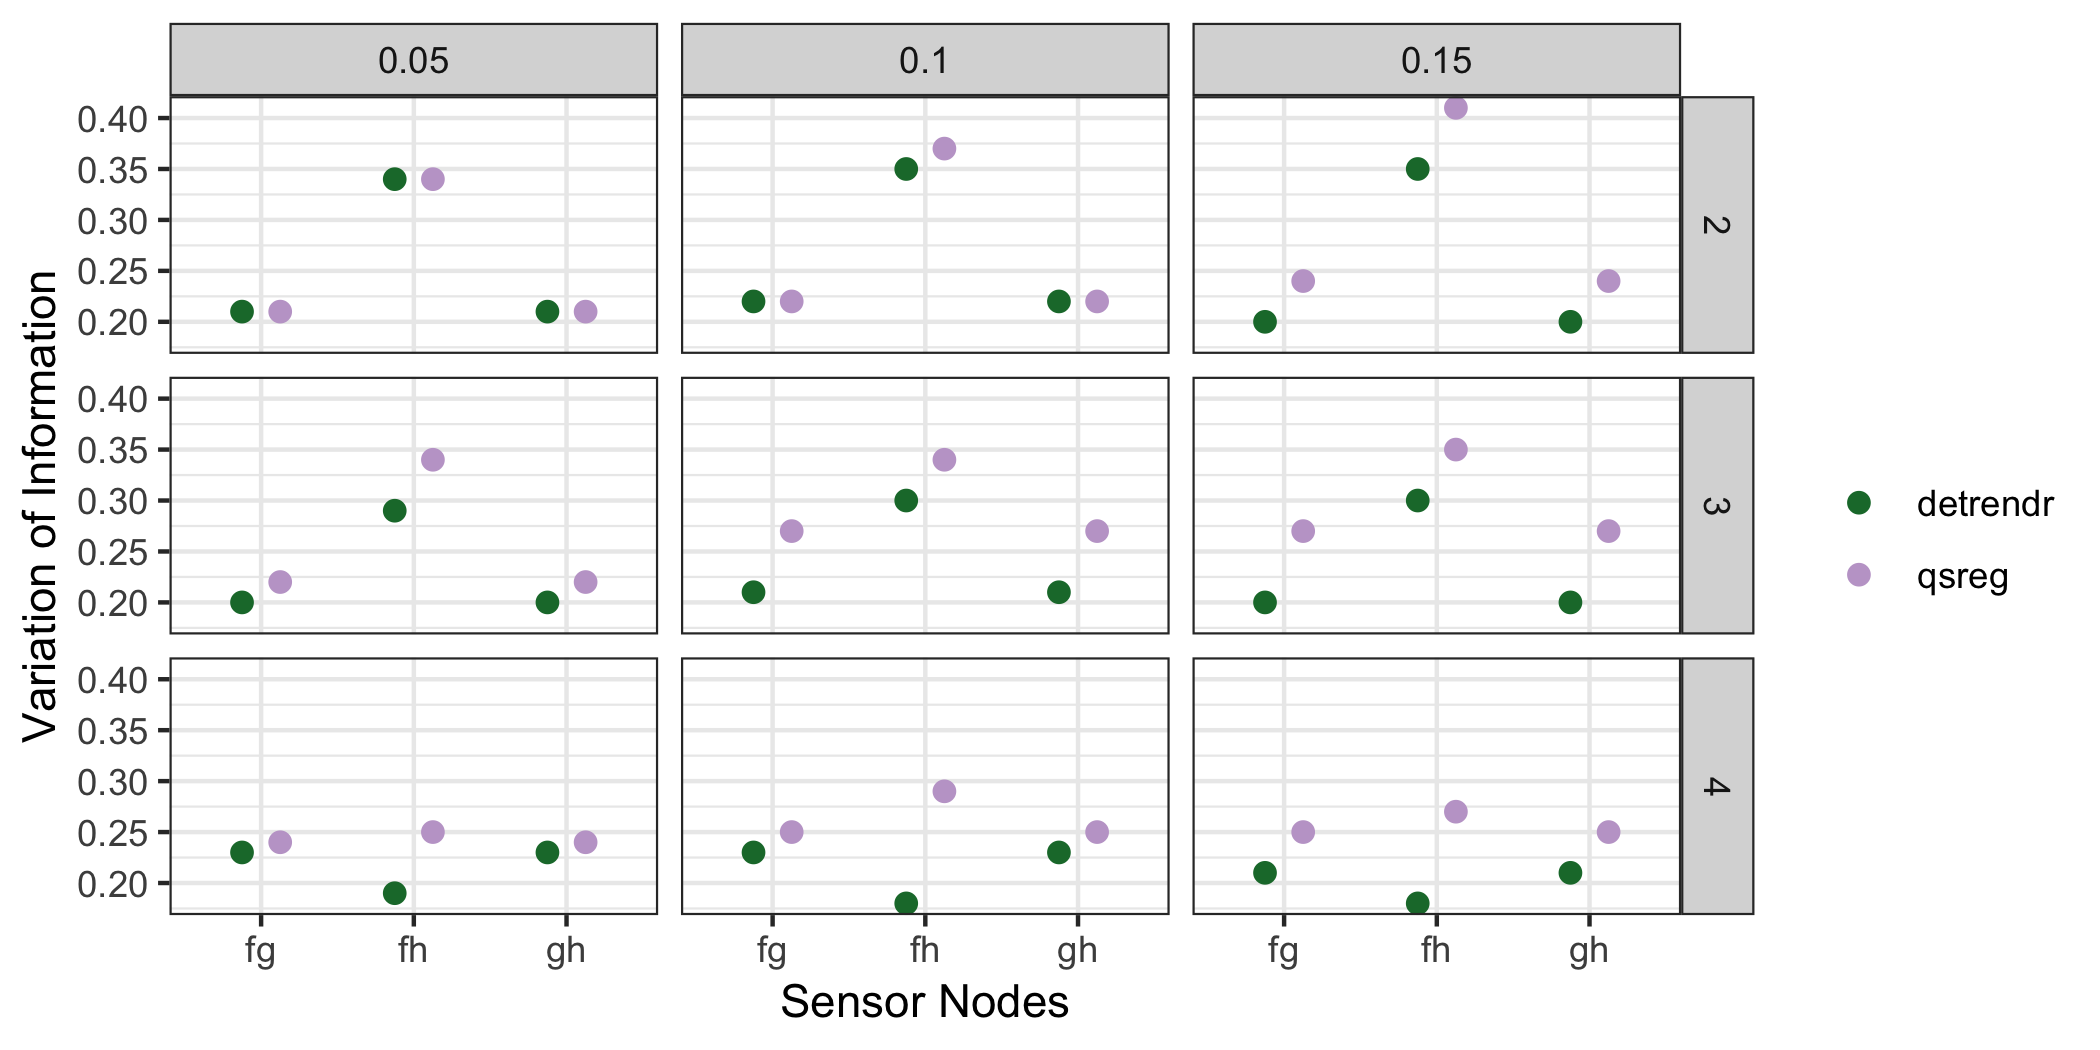
\includegraphics[width = .9\linewidth]{Figures/VI_app_short.png}
		\caption{Variation of Information between sensors by method (color), quantile (columns) and threshold MAD multiple (rows).}
		\label{fig:vi}
	\end{figure}
	
	Our windowed \texttt{detrend\_eBIC} method was used to removed the baseline drift from the total dataset consisting of 86,401 observations per node. The VI scores for the full dataset were 0.36, 0.24, and 0.41 for sensors a and b, a and c, and b and c, respectively. The complete confusion matrices for the nodes using a MAD multiple of 5 for the threshold is given in Table 1. 
		
	\begin{figure}
		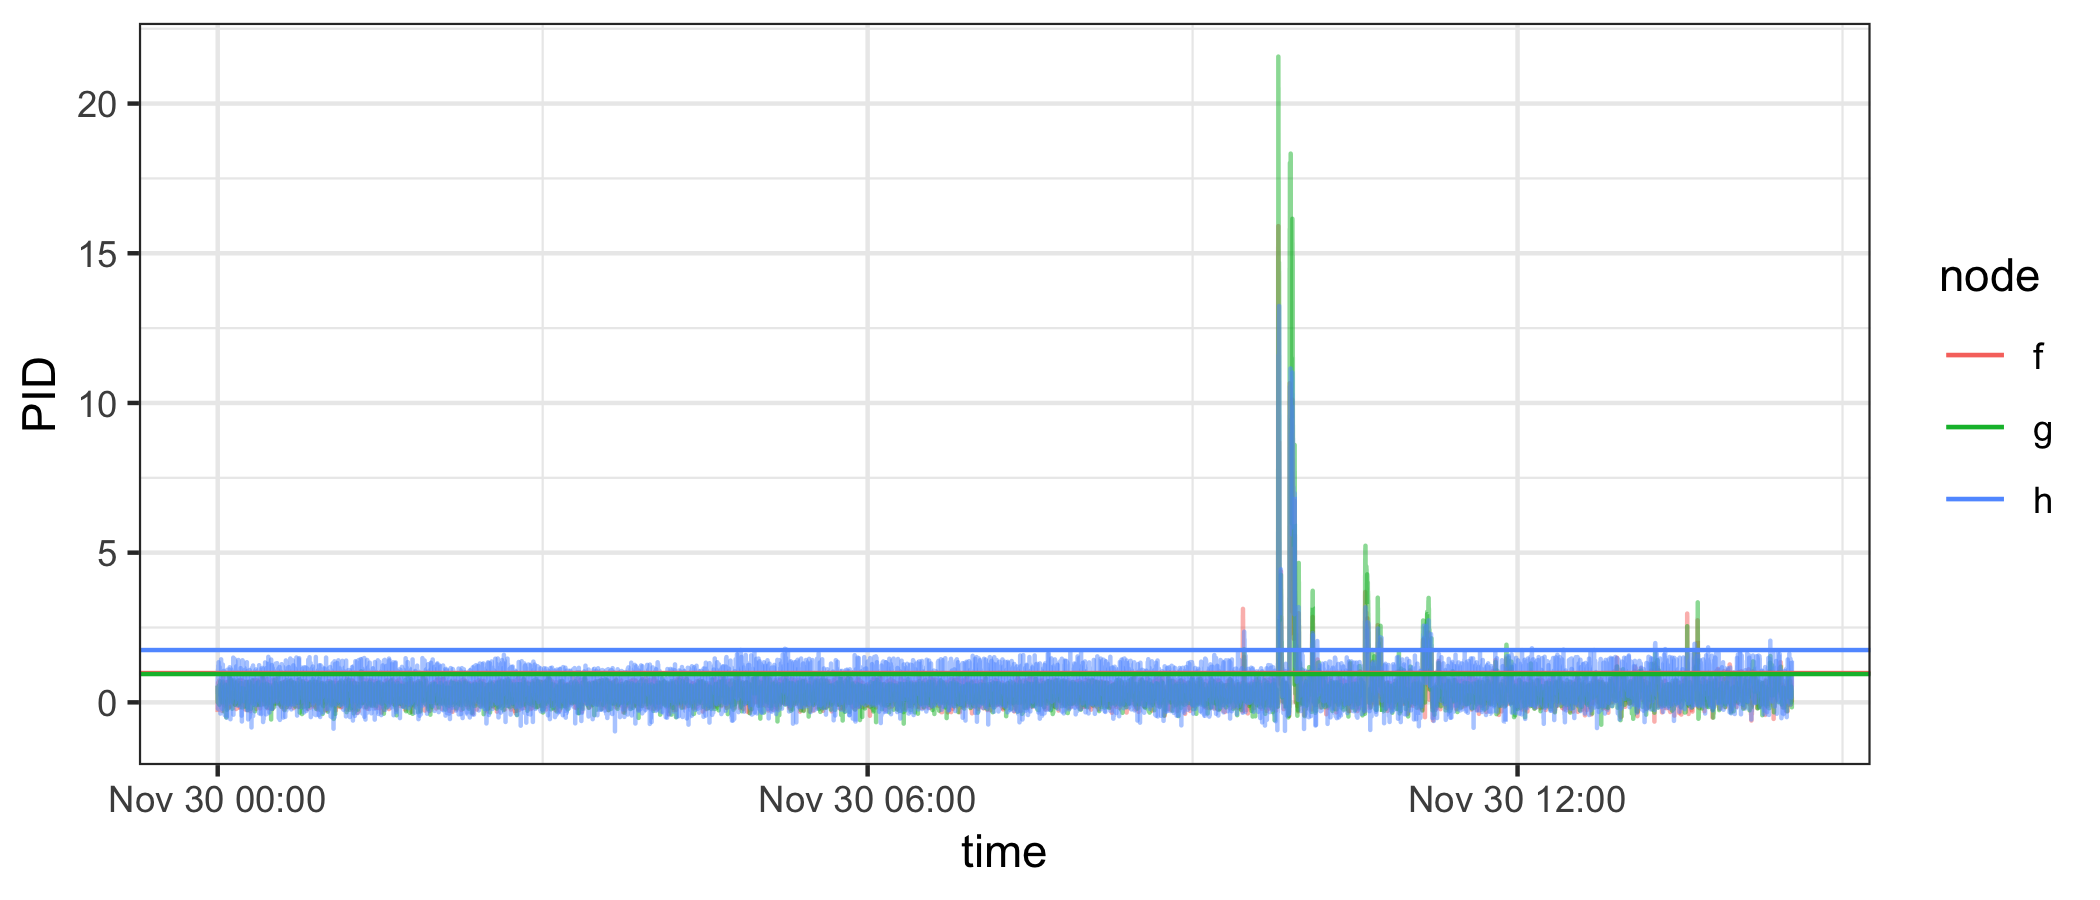
\includegraphics[width = \linewidth]{Figures/corrected_data.png}
		\caption{Low cost sensor data after drift removal using windowed detrend with eBIC.}
	\end{figure}

	%latex.default(conf, file = "../Manuscript/full_confusion_detrend.tex",     rowlabel = "", rowname = c("f = 0", "f = 1", "f=0", "f=1"),     cgroup = c("h = 0", "h = 1"), rgroup = c("tau=0.05", "tau=0.1"),     n.rgroup = c(2, 2), colheads = rep(c("g = 0", "g = 1"), 2),     n.cgroup = c(2, 2), caption = "Confusion matrices for 3 SPod nodes after baseline removal (n=52322).")%
\begin{table}[!tbp]
\caption{Confusion matrices for 3 SPod nodes after baseline removal (n=52322).\label{conf}} 
\begin{center}
\begin{tabular}{lrrcrr}
\hline\hline
\multicolumn{1}{l}{\bfseries }&\multicolumn{2}{c}{\bfseries h = 0}&\multicolumn{1}{c}{\bfseries }&\multicolumn{2}{c}{\bfseries h = 1}\tabularnewline
\cline{2-3} \cline{5-6}
\multicolumn{1}{l}{}&\multicolumn{1}{c}{g = 0}&\multicolumn{1}{c}{g = 1}&\multicolumn{1}{c}{}&\multicolumn{1}{c}{g = 0}&\multicolumn{1}{c}{g = 1}\tabularnewline
\hline
{\bfseries tau=0.05}&&&&&\tabularnewline
~~f = 0&$51641$&$222$&&$1$&$  9$\tabularnewline
~~f = 1&$   23$&$190$&&$7$&$229$\tabularnewline
\hline
{\bfseries tau=0.1}&&&&&\tabularnewline
~~f=0&$51639$&$231$&&$1$&$  9$\tabularnewline
~~f=1&$   23$&$187$&&$7$&$225$\tabularnewline
\hline
\end{tabular}\end{center}
\end{table}
	
	
%% ----------------------------------------------------------------------
%% Conclusion and Discussion
%% ----------------------------------------------------------------------	
\section{Conclusion and Discussion}
\label{sec:discussion}

	We have expanded the quantile trend filtering method by implementing a non-crossing constraint and a new algorithm for processing large series, and proposing a modified criteria for smoothing parameter selection. Furthermore we have demonstrated the utility of quantile trend filtering in both simulations and applied settings. Our ADMM algorithm for large series both reduces the computing time and allows trends to be estimated on series that cannot be estimated simultaneously while our scaled extended BIC criteria was shown to provided better estimated of quantile trends in series with and without a signal component. We have also shown that the baseline drift in low cost air quality sensors can be removed through estimating quantile trends.
	 
	In the future, quantile trend filtering could be extended to observations measured at non-uniform spacing by incorporating the distance in covariate spacing into the differencing matrix. It could also be extended to estimate smooth spatial trends by a similar adjustment to the differencing matrix based on spatial distances between observations. 
	
	\label{sec:conc}
	
	
	\bigskip
	\begin{center}
		{\large\bf SUPPLEMENTARY MATERIAL}
	\end{center}
	
	\begin{description}
		
		\item[R-package for detrend routine:] R-package detrendr containing code to perform the diagnostic methods described in the article. (GNU zipped tar file)
				
	\end{description}
	
	
	\bibliographystyle{asa}
	\bibliography{detrendify}
	
\end{document}

